\chapter{
  High Granularity Calorimeter Upgrade
 }\label{ch_hgcal}

By the start of Run4 period of proton-proton collision
at \gls{LHC}, the collision energy is expected to
reach its full design limit of 14 \TeV{} and
commissioning of \gls{HL-LHC} is expected to
increase the luminosity by 10 times and
integrated luminosity collected by the end of Run5 will be 3000 \fbinv{}.

With increased luminosity the \gls{CMS} detector will get
higher dose of radiation and average number of pileup interactions
will be of the order \( O(140) \) and endcap calorimeters \gls{ECAL} and \gls{HCAL} will suffer
irreparable damage due to the much higher radiation dose received
from increased luminosity in those regions.
The \gls{HGCAL} is an upgrade that will replace current endcap calorimeters
\gls{ECAL} and \gls{HCAL}.
\gls{HGCAL} is expected to be completed, and installed
during \gls{LS3} (2026--2028).

This chapter will discuss broadly the design
of \gls{HGCAL}, especially the scintillator section of the \gls{HGCAL}
and studies done at \gls{NICADD} towards its upgrade,
for complete design see the \gls{TDR}~\cite{cms-hgcal-tdr}.

\section{
  Technical Design and Requirements
 }\label{ch_hgcal:technical-design}

As mentioned the \gls{HGCAL} will replace current endcap \gls{ECAL} and
\gls{HCAL}, Figure~\ref{fig:cms-hgcal-quadrant-layout}
shows exactly where the new detector will pe placed. The right image in the
Figure~\ref{fig:cms-hgcal-quadrant-layout} shows side view (\( z-r \) plane)
of the detector, starting from the left i.e.~innermost layers is
\gls{CE-E} whose active layers are made of all silicon cells
(\( \approx 0.5-1 \cm{}^2\)), then
majority of the detector in longitudinal length is \gls{CE-H}
whose starting few active layers are also all silicon cells, and
then its mixed with silicon cells in lower rings of the
layer and the scintillator tiles (\( \approx 5-31 \cm{}^2\)) in the rest.
Silicon is radiation hard material i.e.~the response of silicon cells
will not degrade under high rate of radiation dose, but
silicon is also expensive and for such high cell count in \gls{HGCAL}
it significantly increase the budget of the project, for this
reason scintillator tiles are used wherever radiation doses are low.
Some of the main reasons for high cell count, lateral and longitudinal granularity
are to preserve energy resolution after 3000 \fbinv{}, precision
timing measurement of the showers to reject energy deposit from pileup, and
been able to observe narrower jets with \( R = 0.2 \).
To be able to deliver these requirements both silicon cells and scintillator tiles
need to have good \gls{SNR} even after 3000 \fbinv{}.

\begin{figure}[!ht]
  \centering
  \begin{minipage}[c]{0.49\textwidth}
    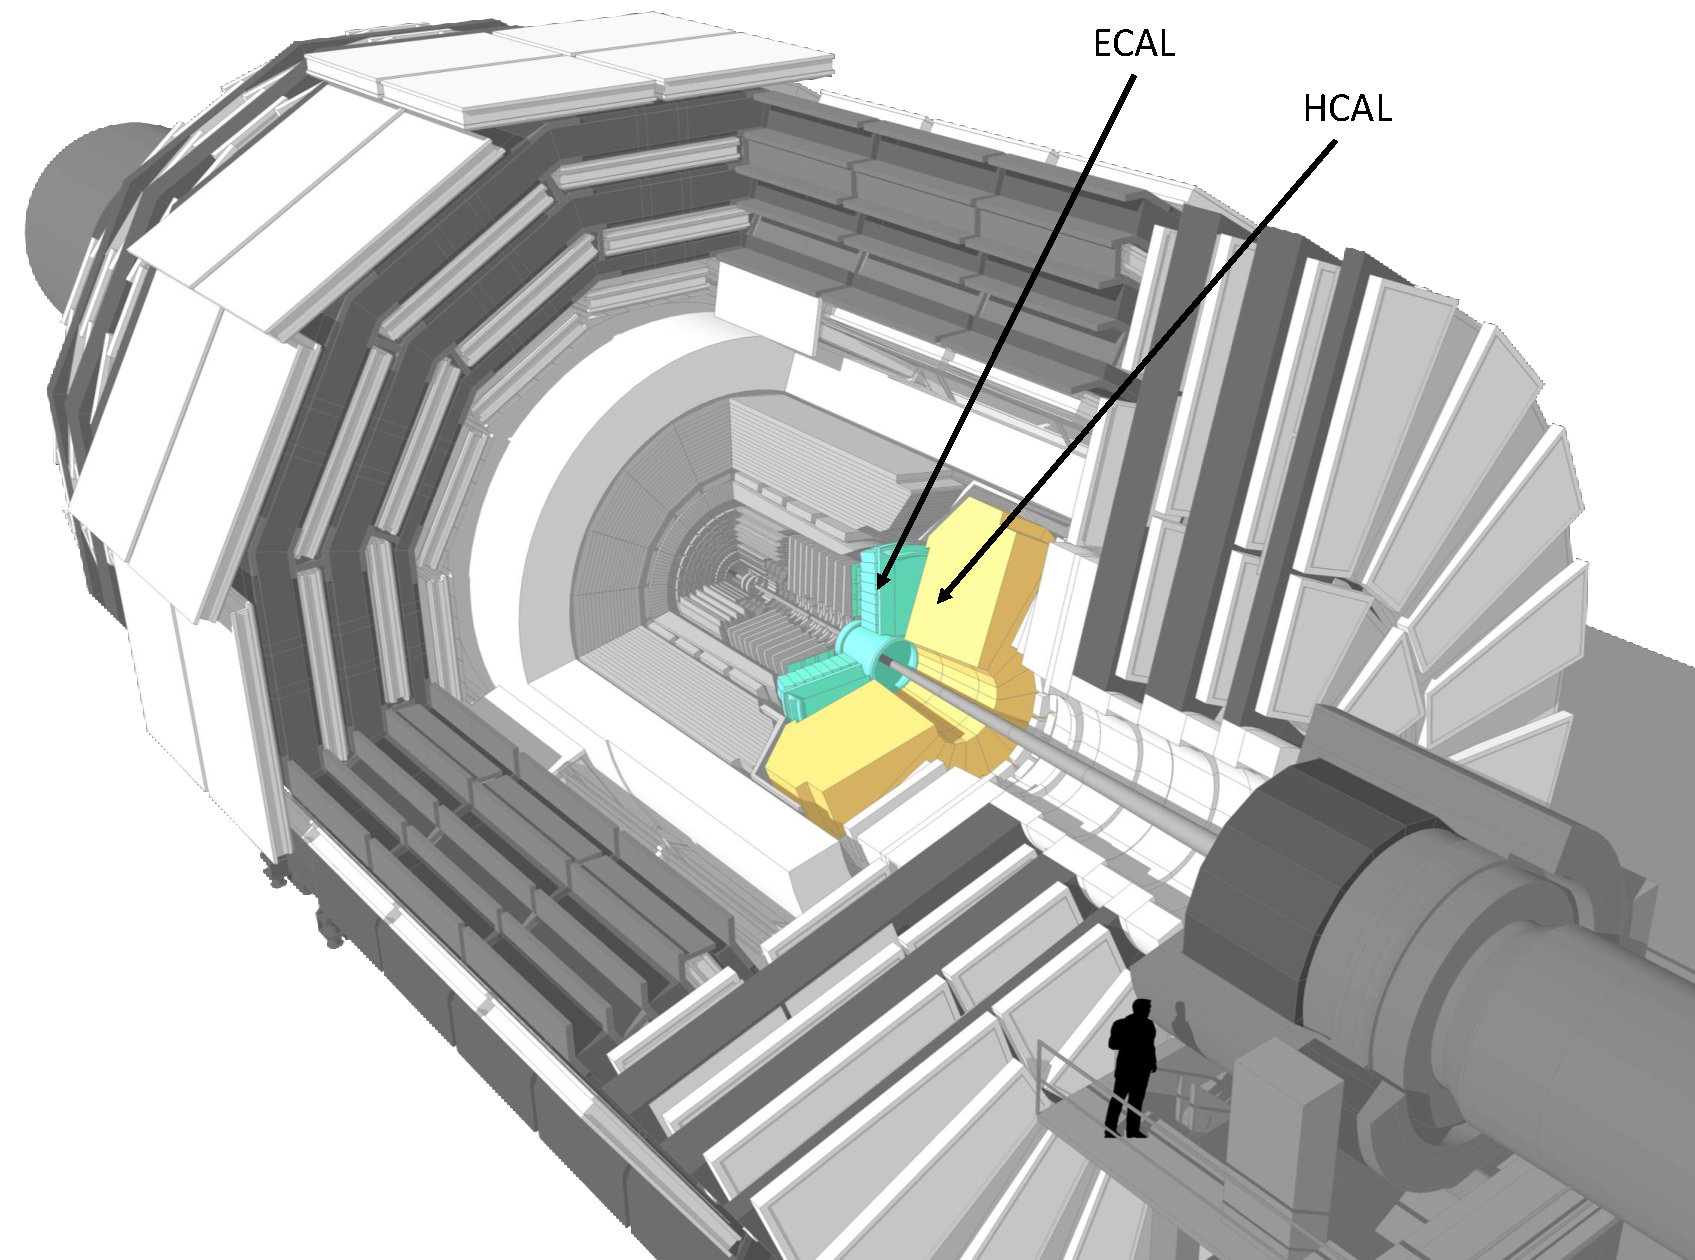
\includegraphics[width=\textwidth]{figures/hgcal/hgcal_place.pdf}
  \end{minipage}
  \begin{minipage}[c]{0.49\textwidth}
    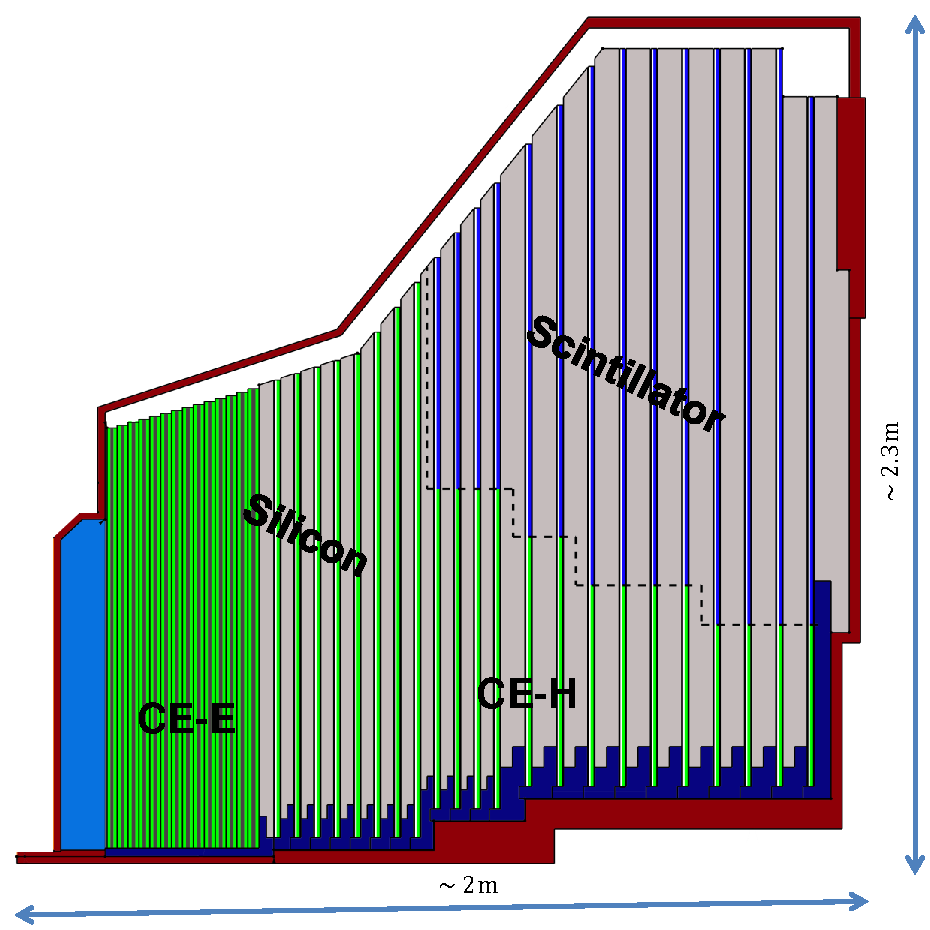
\includegraphics[width=0.9\textwidth]{figures/hgcal/hgcal_quadrant.pdf}
  \end{minipage}
  \caption[Overview of HGCAL position and quadrant view of CE]%
  {Overview of HGCAL position and quadrant view of \gls{CE}. Left image
    shows current endcap \gls{ECAL} and \gls{HCAL} highlighted.
    Right image shows quadrant view of \gls{HGCAL} from the side~\cite{image-cms-hgcal-quadrant-layout,image-cms-hgcal-place}.}%
  \label{fig:cms-hgcal-quadrant-layout}
\end{figure}

\clearpage
\section{
  Scintillator Tiles and SiPMs
 }

Silicon cells will be directly fabricated 8 inch silicon wafers (432
cells) as shown
in Figure~\ref{fig:hgcal-layer-22} as yellow and green colored hexagons,
whereas each scintillator tiles will need to prepared separately
and assembled in the form of ``tileboard'' (about \(8\times 8\) tiles).
Figure~\ref{fig:hgcal-layer-22} shows scintillator
tiles boundary with red grid lines, there are 288
scintillator tiles in
each ring, and each layer has different
number of rings of scintillator tiles with maximum of 40 rings. To reduce
the production cost and assembly complexities scintillator size are
same for every two rings, and ring number is used to identify tile
size, for example R18--19 is the tile size of tiles in ring number 18 and 19.

\begin{figure}[!ht]
  \centering
  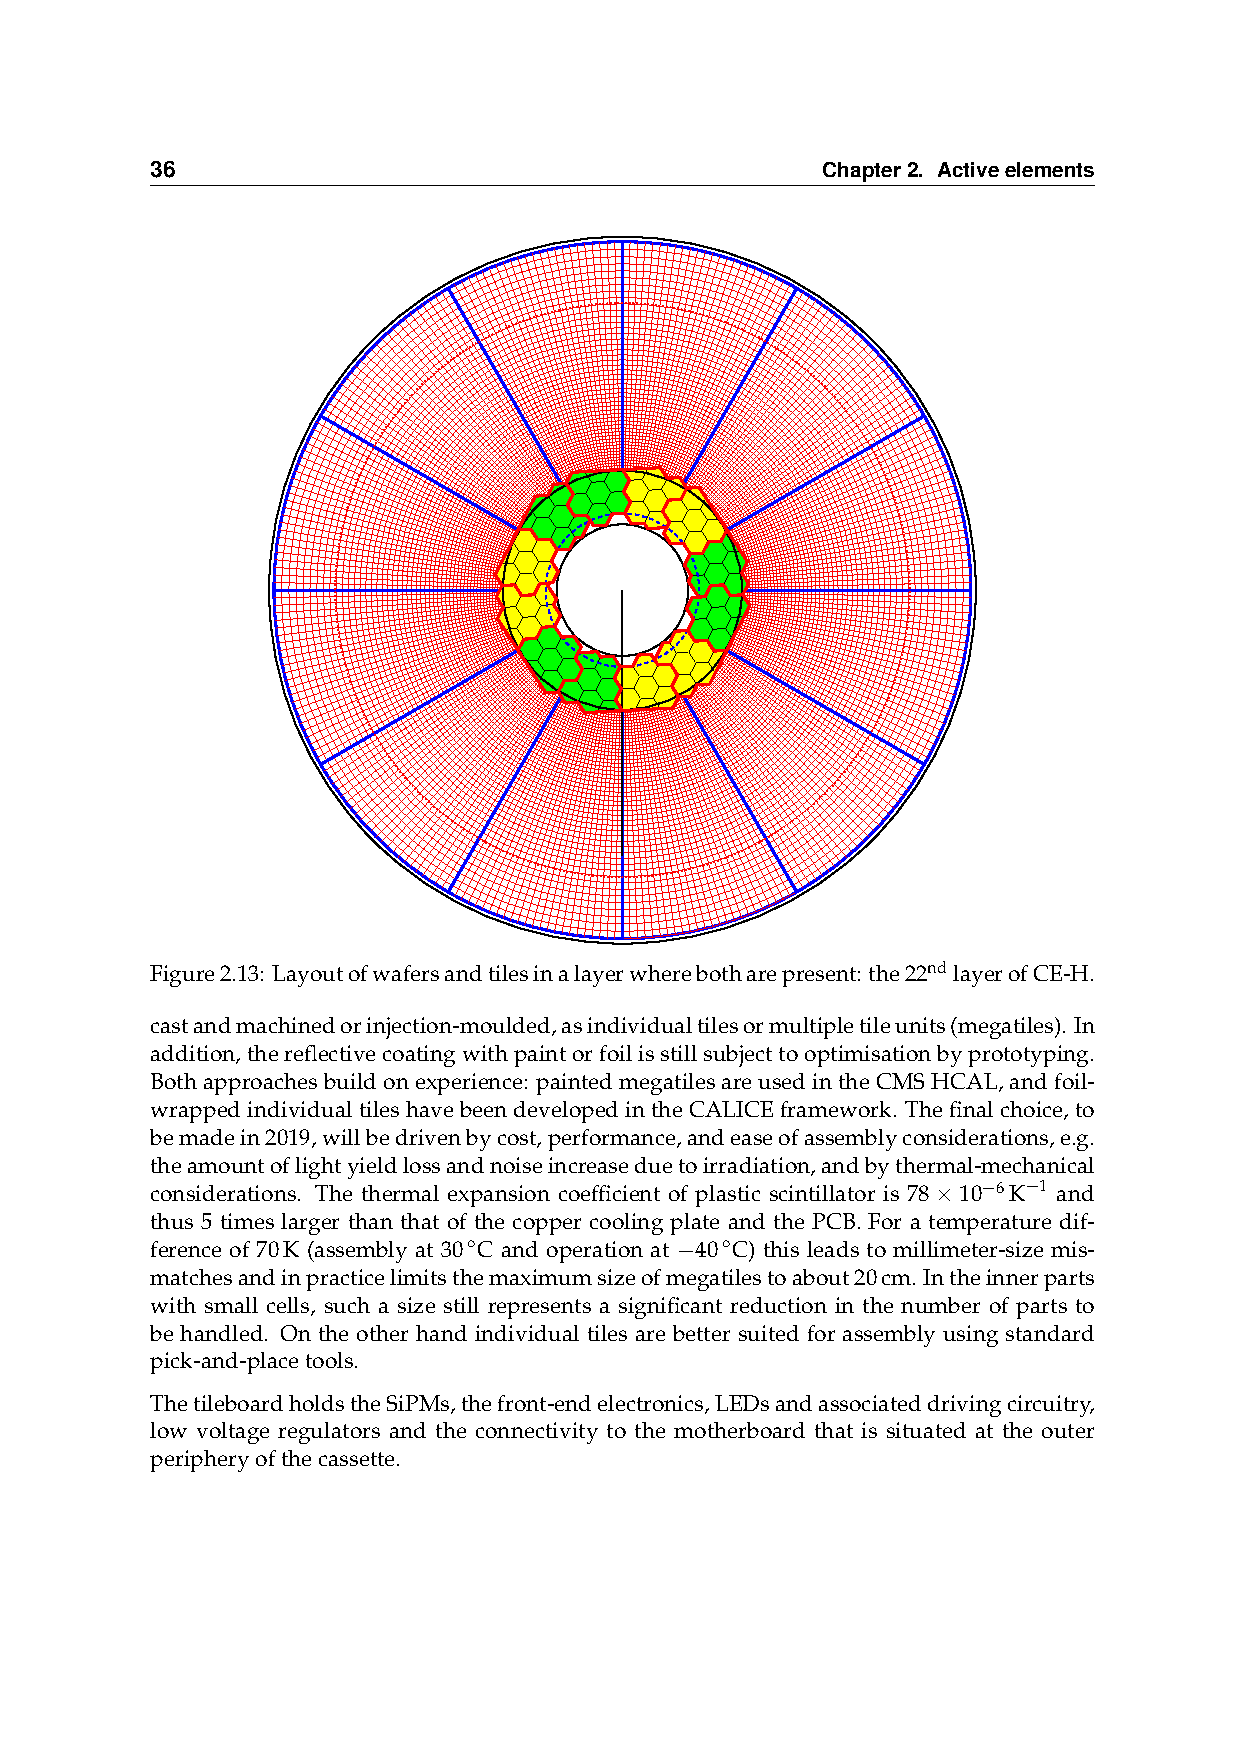
\includegraphics[trim={129 389 127 113},clip,width=0.5\textwidth]{figures/hgcal/page36_TDR_HGCAL.pdf}
  \caption[CE-H mixed layer 22]
  {CE-H mixed layer 22. Yellow and green hexagons are the
    8 inch silicon modules and the red grid lines shows
    11,520 (40 rings) scintillator tiles.~\cite{cms-hgcal-tdr}.}%
  \label{fig:hgcal-layer-22}
\end{figure}

\subsection{
  Scintillator Materials
}

Materials which scintillates i.e.~emits light
whenever a ionizing radiation passes through it.
Scintillator material can be crystals (current barrel and endcap
\gls{ECAL}), liquid or plastic and are broadly divided into two
categories organic or inorganic scintillators.
\gls{HGCAL} will make use of organic plastic scintillator, and the most
commonly used scintillator of this type are \gls{PVT} and \gls{PS}.
\gls{PVT} and \gls{PS} are base material and
by themselves cannot serve the purpose of scintillator tiles for couple of
reasons the light emitted is at lower wavelengths (ultraviolet)
and they are barely transparent to this light,
for these reasons they have small percentage of dopants added
which absorbs the scintillation light and re-emits at larger wavelengths (visible)
and a second dopant is added to further increase the attenuation length of
the light emitted, so that light can be collected and coupled with light
detection system.

\gls{PVT} based scintillator will be referred to as ``cast'' scintillator,
and they are usually available in large sheets from vendors and
need to be machined to make dimple and reduce size.
\gls{PST} based scintillator are called ``injection molded'' scintillator
because they are molded into desired tile shape.

Cast scintillators are generally brighter (in terms of light output)
than injection molded scintillators, but the cost of
cast scintillator per area is generally higher.
Choice of scintillator in addition to \gls{SiPM}, which will discuss next
impacts how will optimizing
cost and still retain good \gls{SNR} for lifetime of \gls{HGCAL}.

\subsection{
  SiPMs
}

\gls{SiPM} is a device that convert incident photon to electric
current with large gain of \( 10^5 \) to \( 10^6 \) electrons.
\gls{SiPM} achieves this by pixels (10\micron{} to 100\micron{} in size)
connected in parallel, where each pixel is a avalanche photodiode (APD)
combined with quenching resistor. \gls{SiPM} of active
area \( 2\mm{}^2 \) with 15\micron{} pixel has approximately 9,000 pixels,
commercially \gls{SiPM} are also known as \gls{MPPC}~\cite{mppc-13360}. Figure~\ref{fig:hgcal-sipm}
shows \gls{SiPM} next to tip of a pen.

\gls{SiPM} operates in reverse bias (Geiger Mode),
with voltage above breakdown \gls{OV}, with linear relationship
between \gls{OV} and gain.
In addition to low operating voltage (\(40-60\) V) the power
consumption is also low, which increases with the number of pixel.
For \gls{HGCAL} Hamamatsu S14160~\cite{mppc-14160} is being considered with
area 2, 4 and \(9\mm{}^2\). Larger area means large signal, but
also means higher power consumption which can be significant given
the granularity of the \gls{HGCAL}.

For \gls{HGCAL} the \glspl{SiPM} will be mounted on \gls{PCB},
and prepared scintillator tiles will be directly glued on
over \glspl{SiPM} with dimple centering on \gls{SiPM}'s active area.

\begin{figure}[!ht]
  \centering
  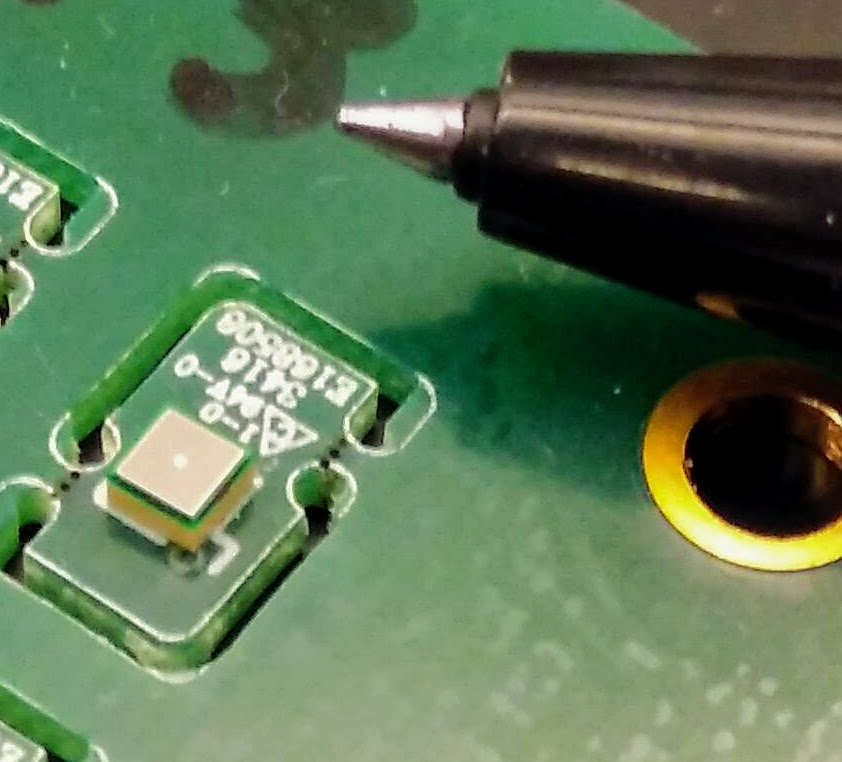
\includegraphics[width=0.4\textwidth]{figures/hgcal/sipm.jpg}
  \caption[SiPM]{SiPM}%
  \label{fig:hgcal-sipm}
\end{figure}

\subsection{
  Scintillator Tiles
}\label{ch_hgcal:scint-tiles}

Scintillator tiles coupled directly with \gls{SiPM} alone can not provide
sufficient \gls{SNR} to reject noise with certainty, additionally
the response will be non-uniform centered at \gls{SiPM}. Higher
signal and uniform response, both can be achieved by coating or wrapping in reflective
material~\cite{niu-sipm-on-tile}. \gls{ESR}
is a multi-layer highly reflective material with 65\micron{} thickness,
and is the material chosen for wrapping scintillator tiles with this.

As visible from Figure~\ref{fig:hgcal-layer-22} the number
of individual tiles in each layer is already very high, and to wrap
100--200 thousand tiles with \gls{ESR} is a very challenging task.
At \gls{NICADD} we are building an automated wrapping machine (Section~\ref{ch_hgcal:wrapping}) to
wrap scintillator tiles with speed and repeatability.
Figure~\ref{fig:hgcal-scintillator-tile} shows the
R18--19 size scintillator tile, Figure~\ref{fig:hgcal-esr-wrapper}
is the \gls{ESR} cut into shape for wrapping R18--19 tiles.

\begin{figure}[!ht]
  \centering
  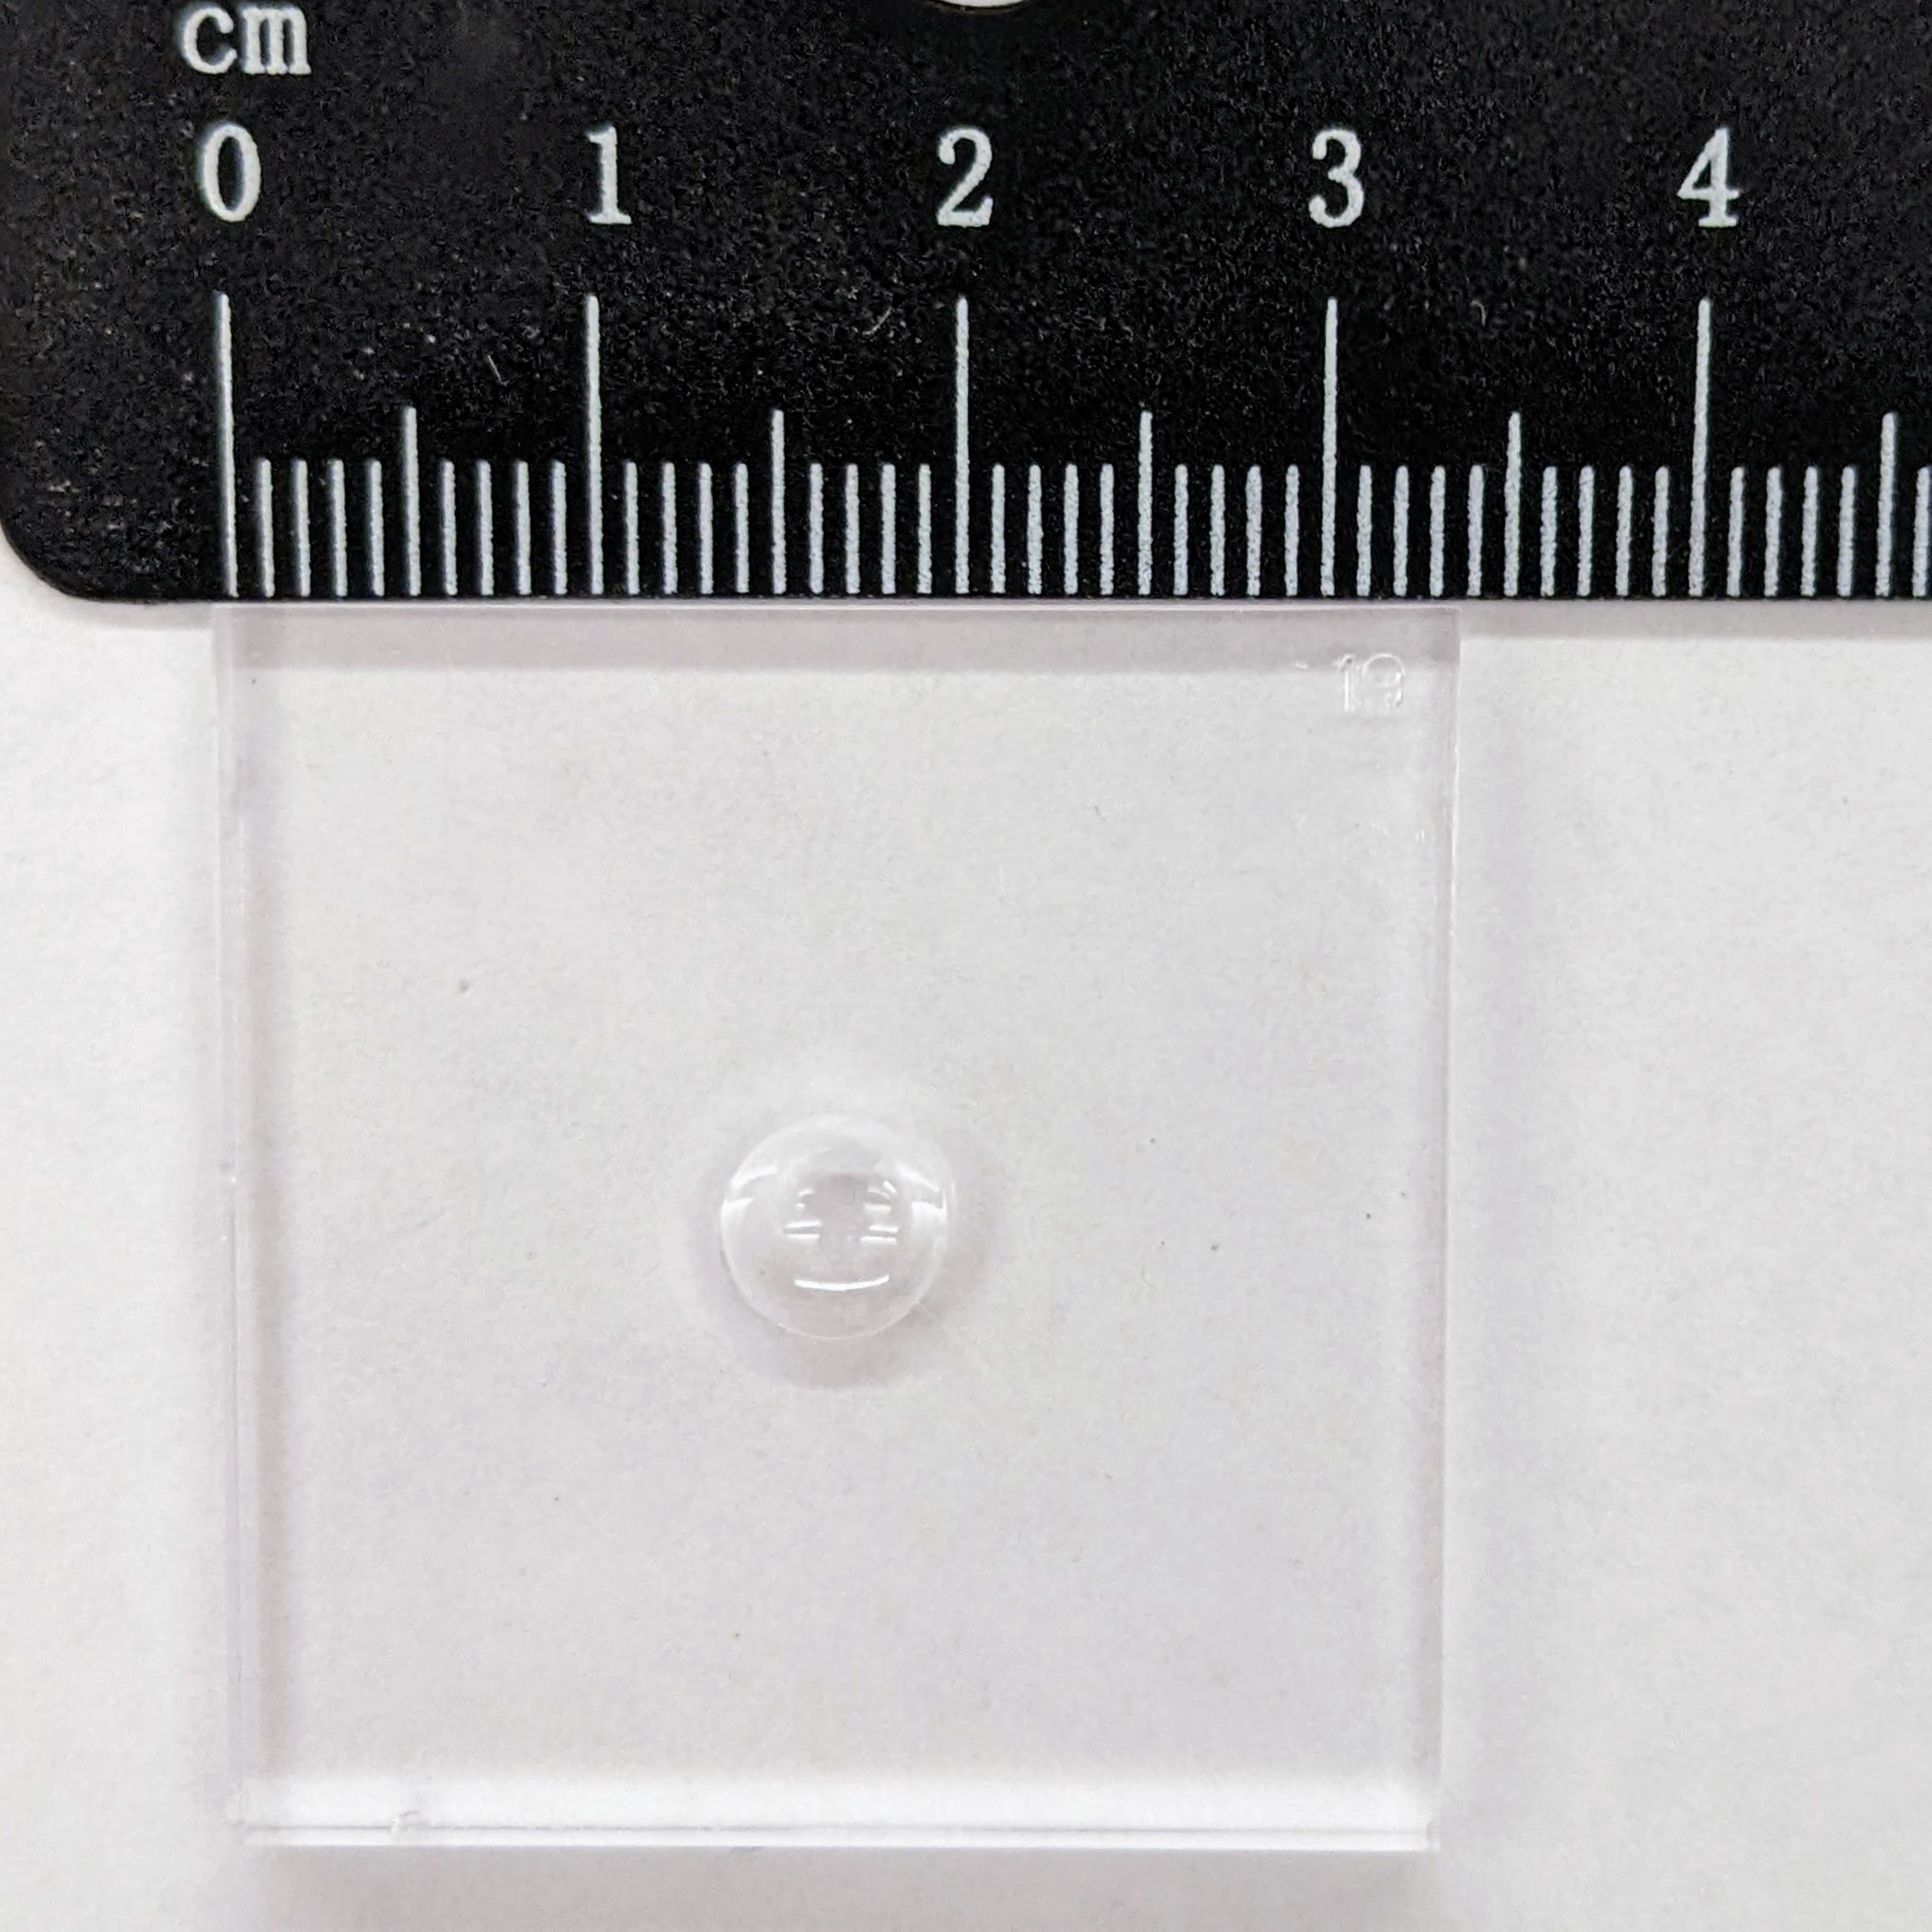
\includegraphics[width=0.5\textwidth]{figures/hgcal/tile_19.jpg}
  \caption[Scintillator tile with dimple]{Scintillator tile with dimple}%
  \label{fig:hgcal-scintillator-tile}
\end{figure}

\begin{figure}[!ht]
  \centering
  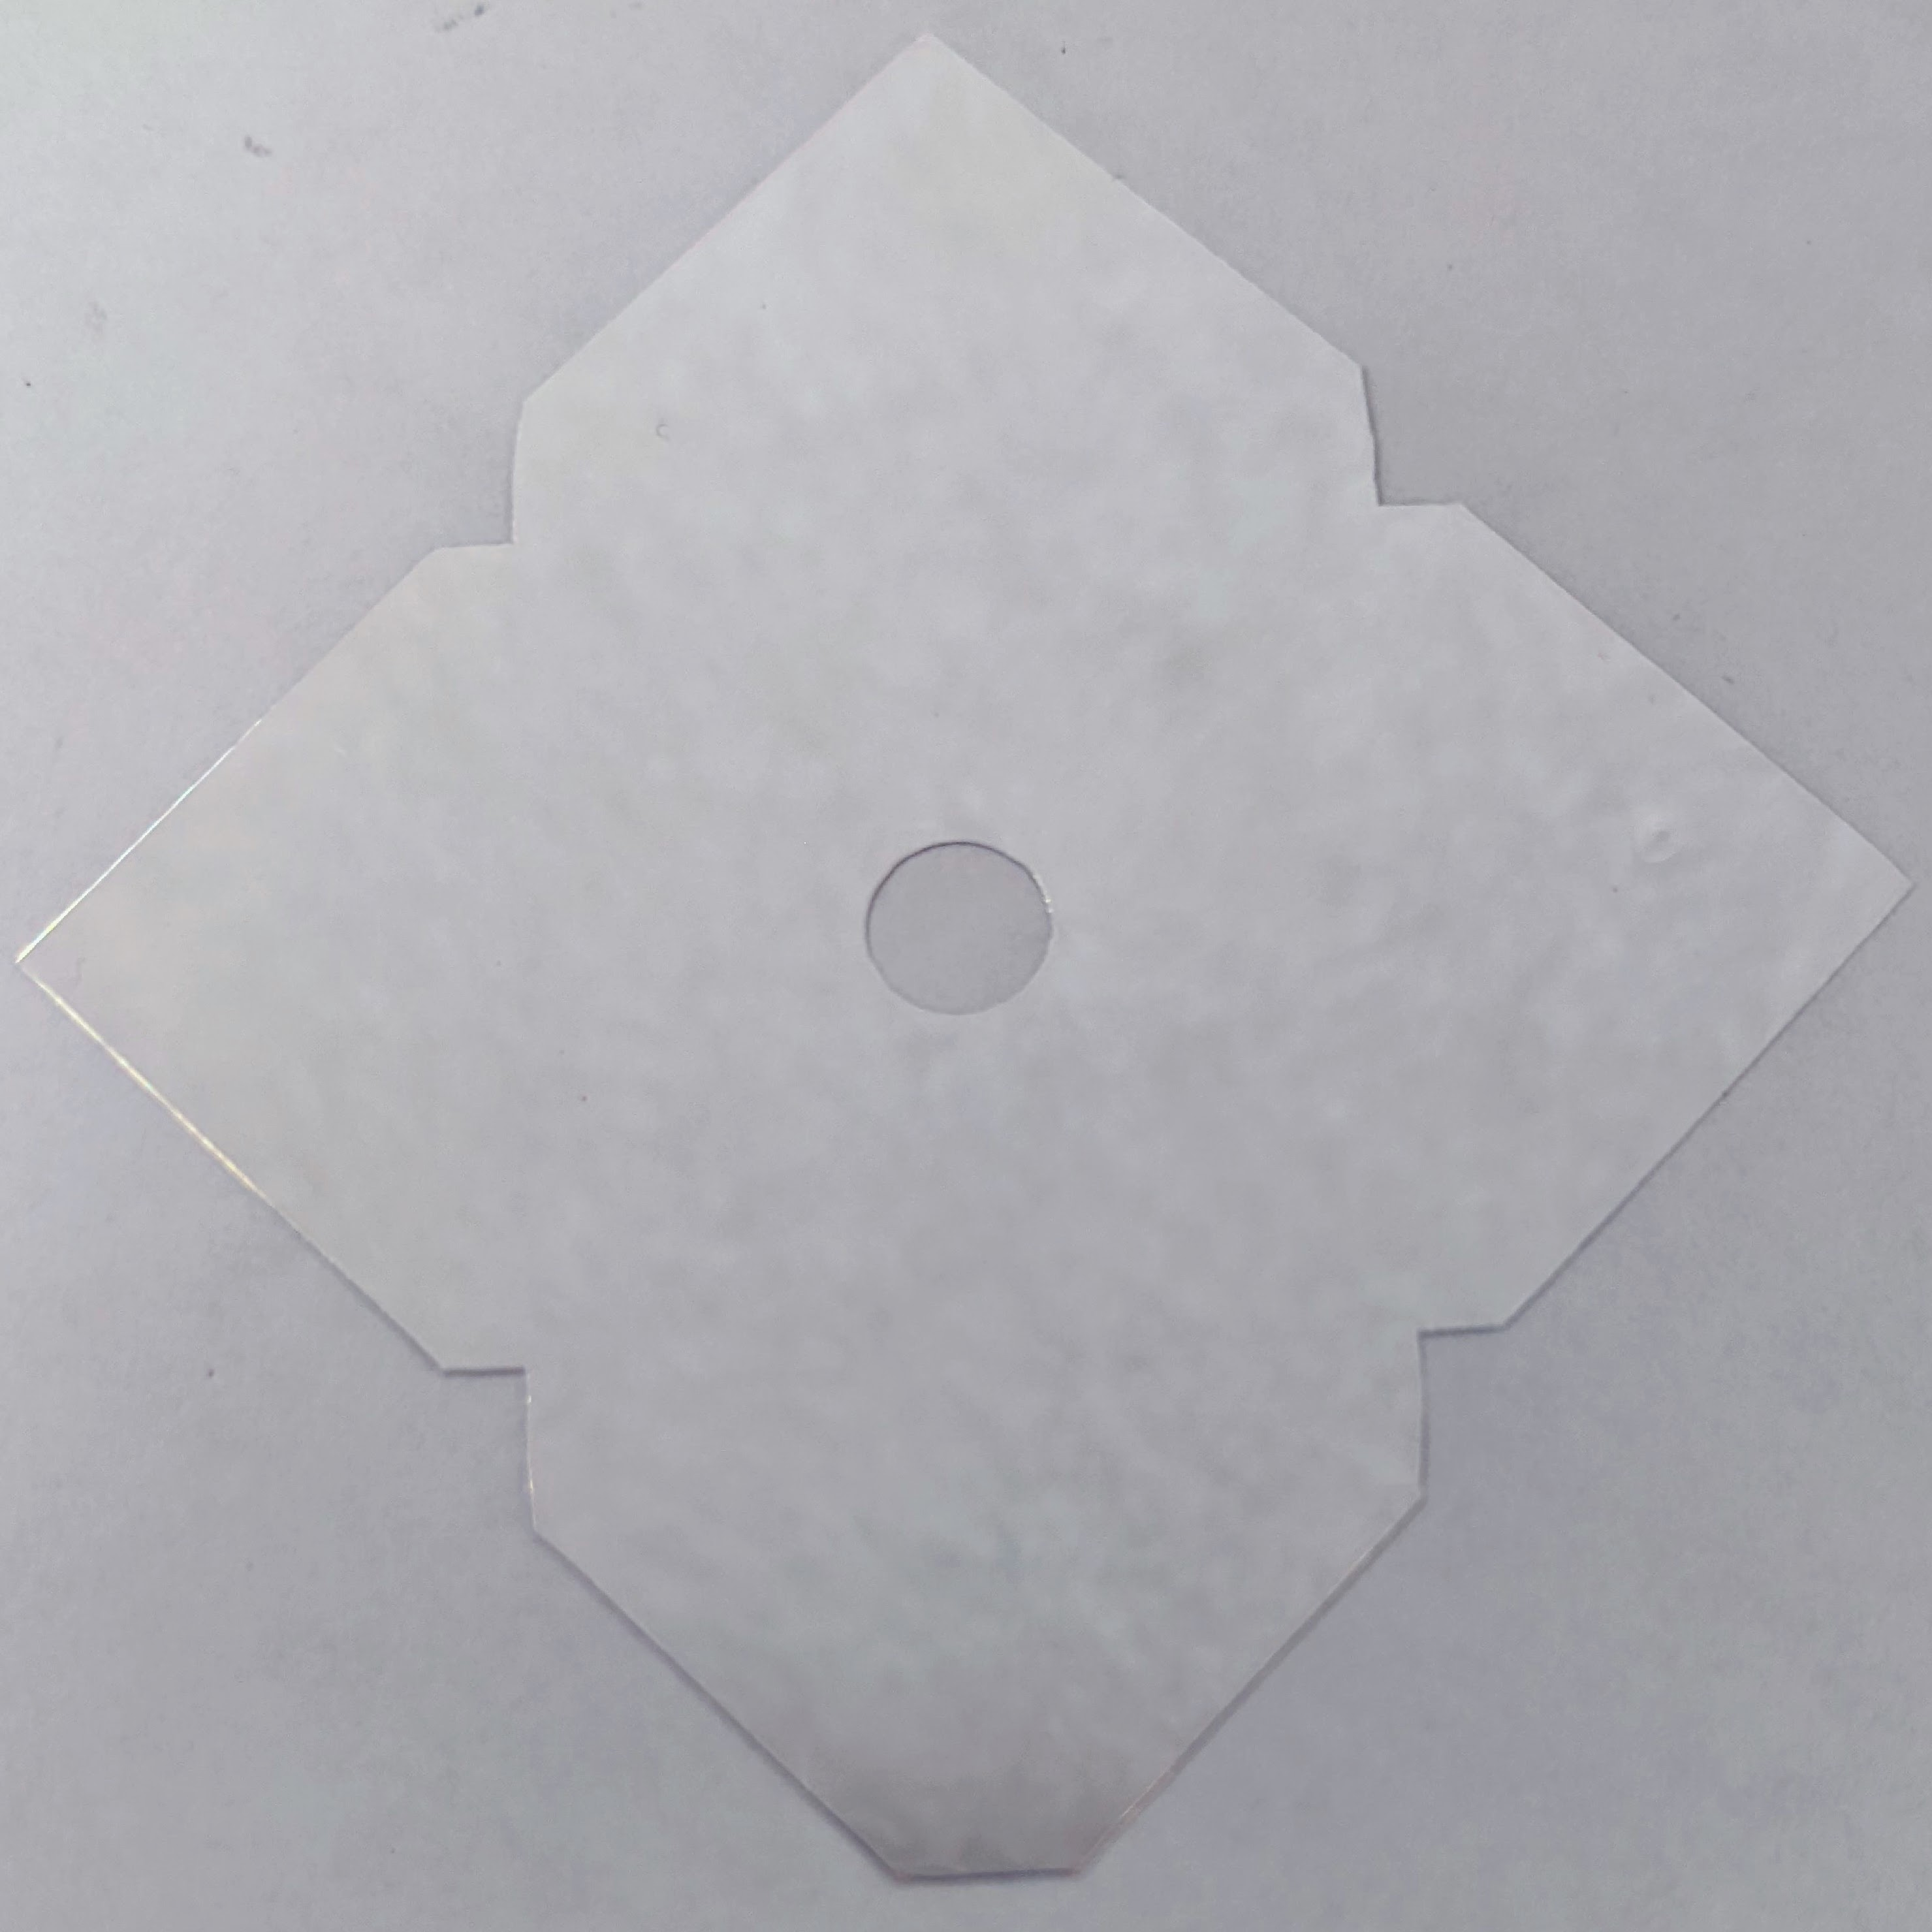
\includegraphics[width=0.5\textwidth]{figures/hgcal/esr_wrapper.jpg}
  \caption[ESR wrapper cut for tile size R18--19]
  {ESR wrapper cut for tile size R18--19}%
  \label{fig:hgcal-esr-wrapper}
\end{figure}

The final wrapped tile in complete automated process
with wrapping machine being developed and build at \gls{NICADD}
is shown in Figure~\ref{fig:hgcal-scintillator-tile-wrapped}.

\begin{figure}[!ht]
  \centering
  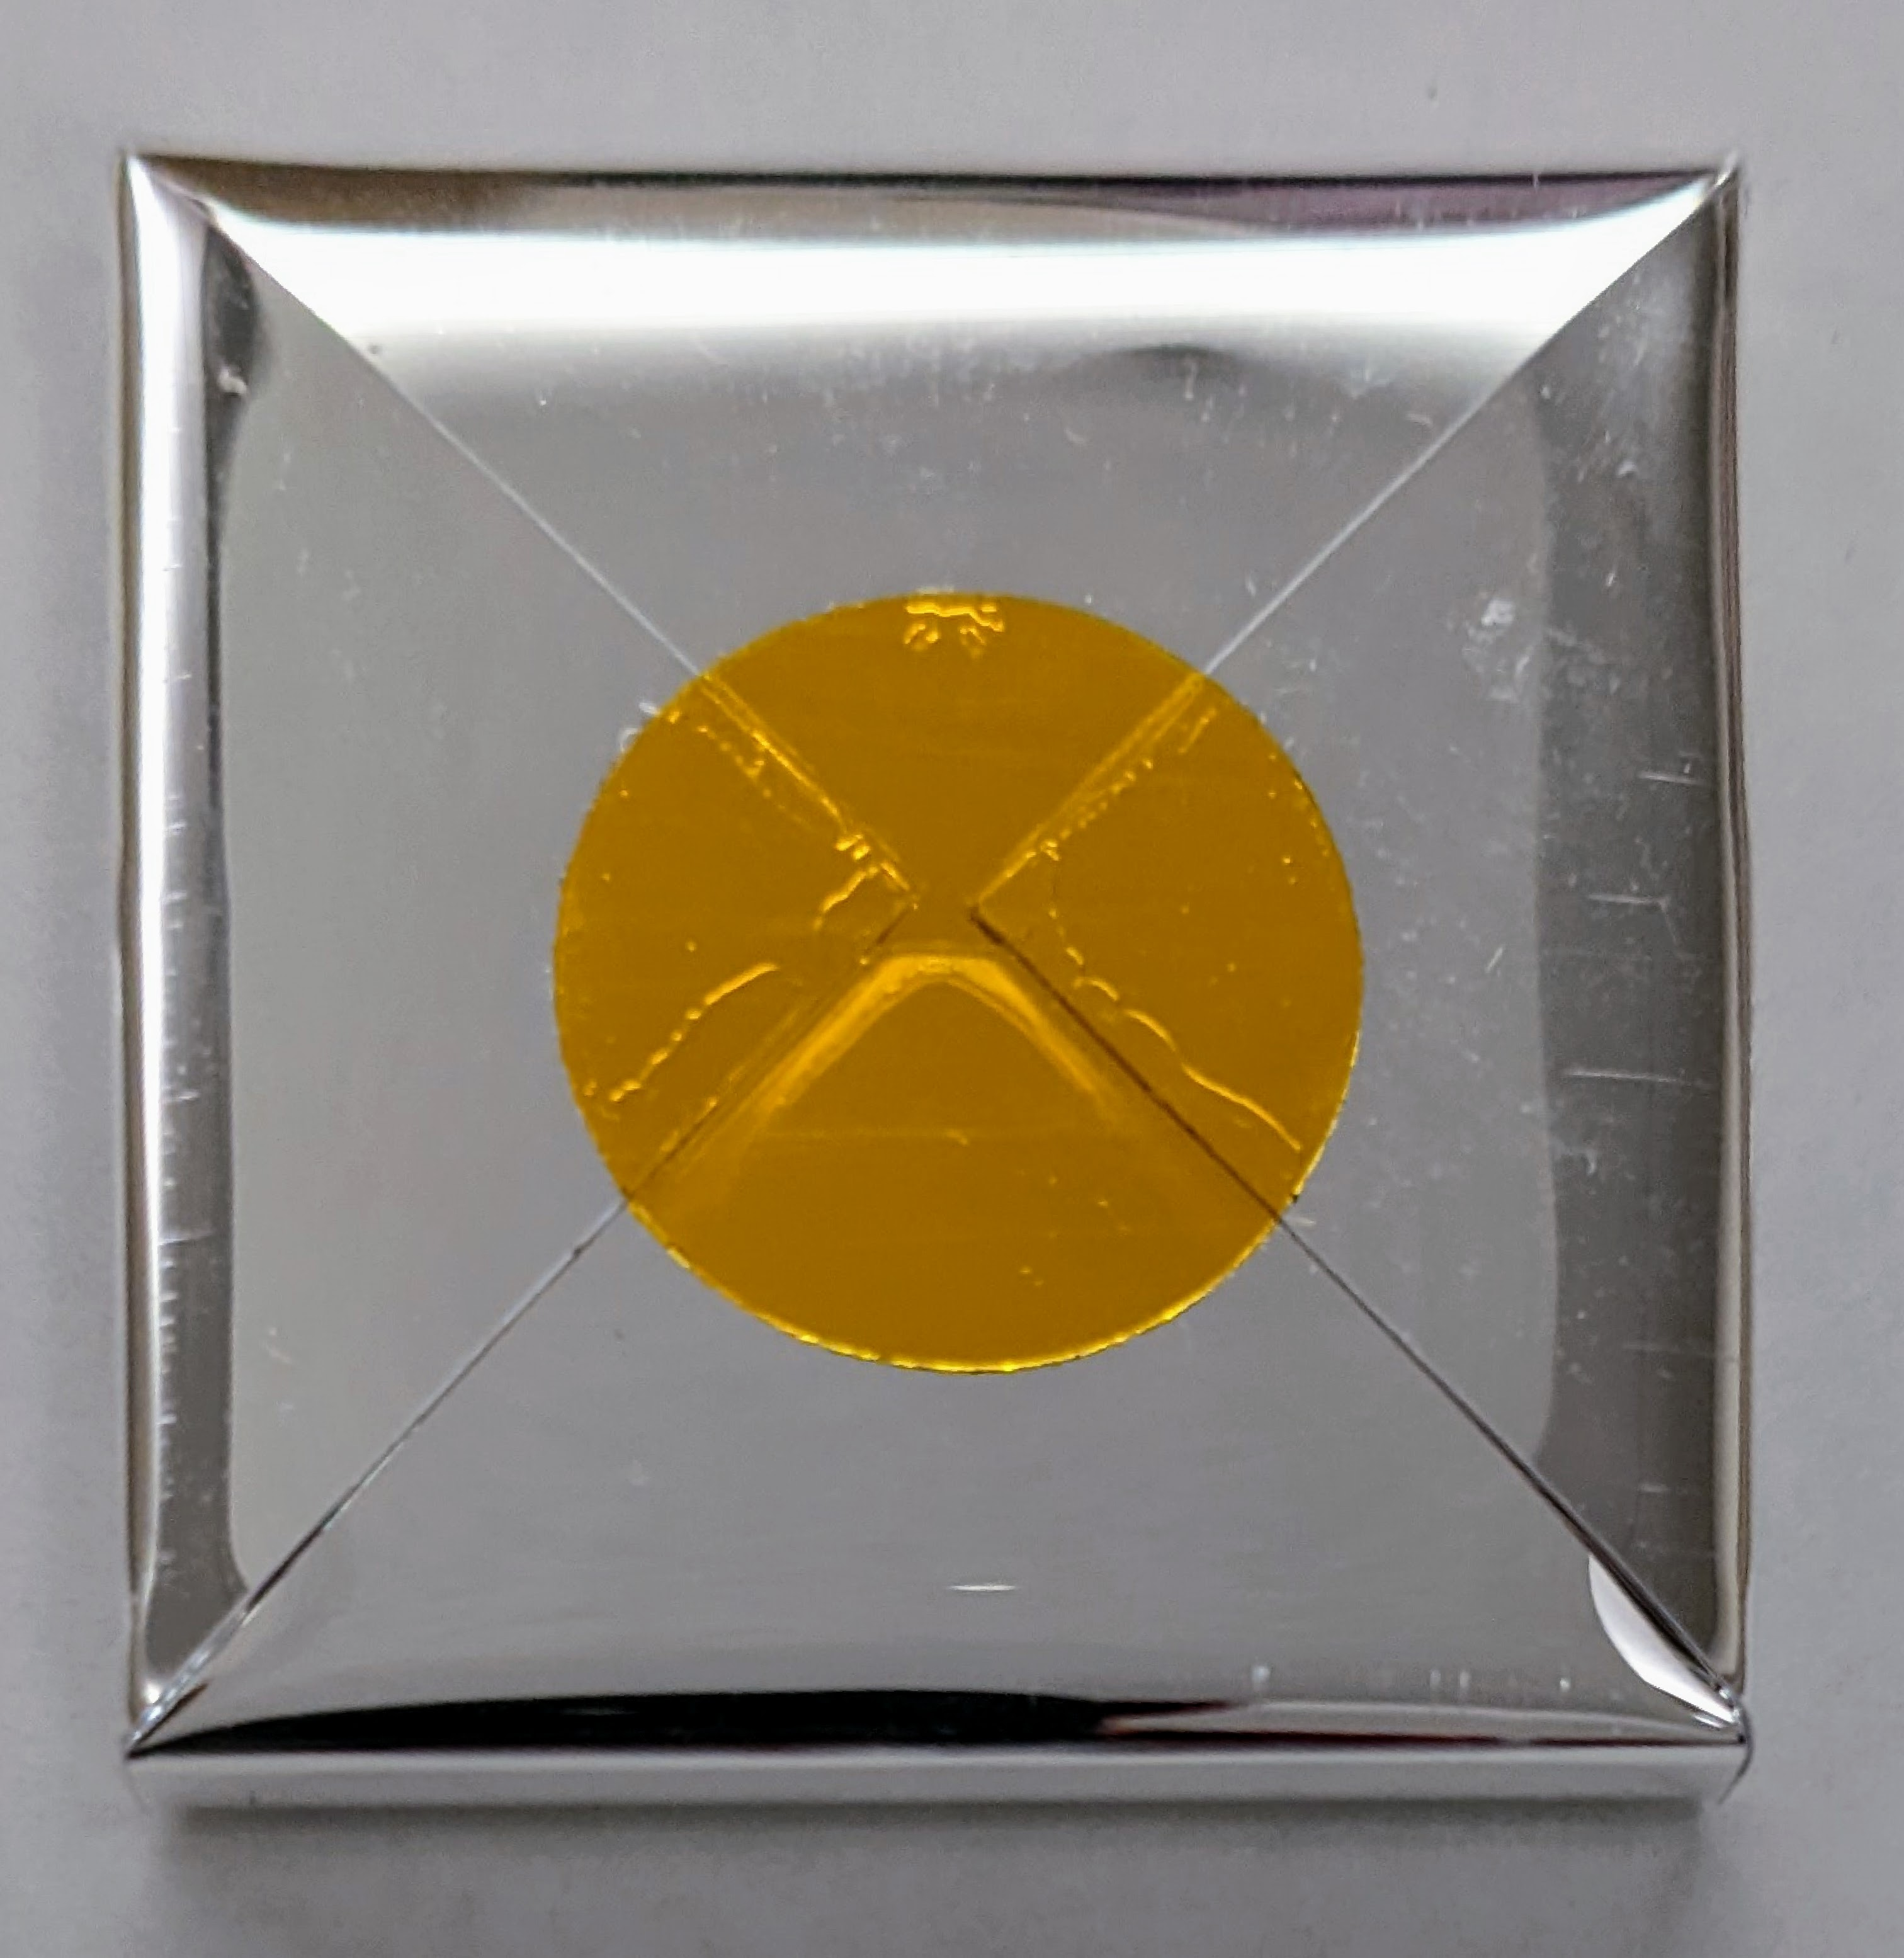
\includegraphics[width=0.4\textwidth]{figures/hgcal/wrapped_tile_up.jpg}
  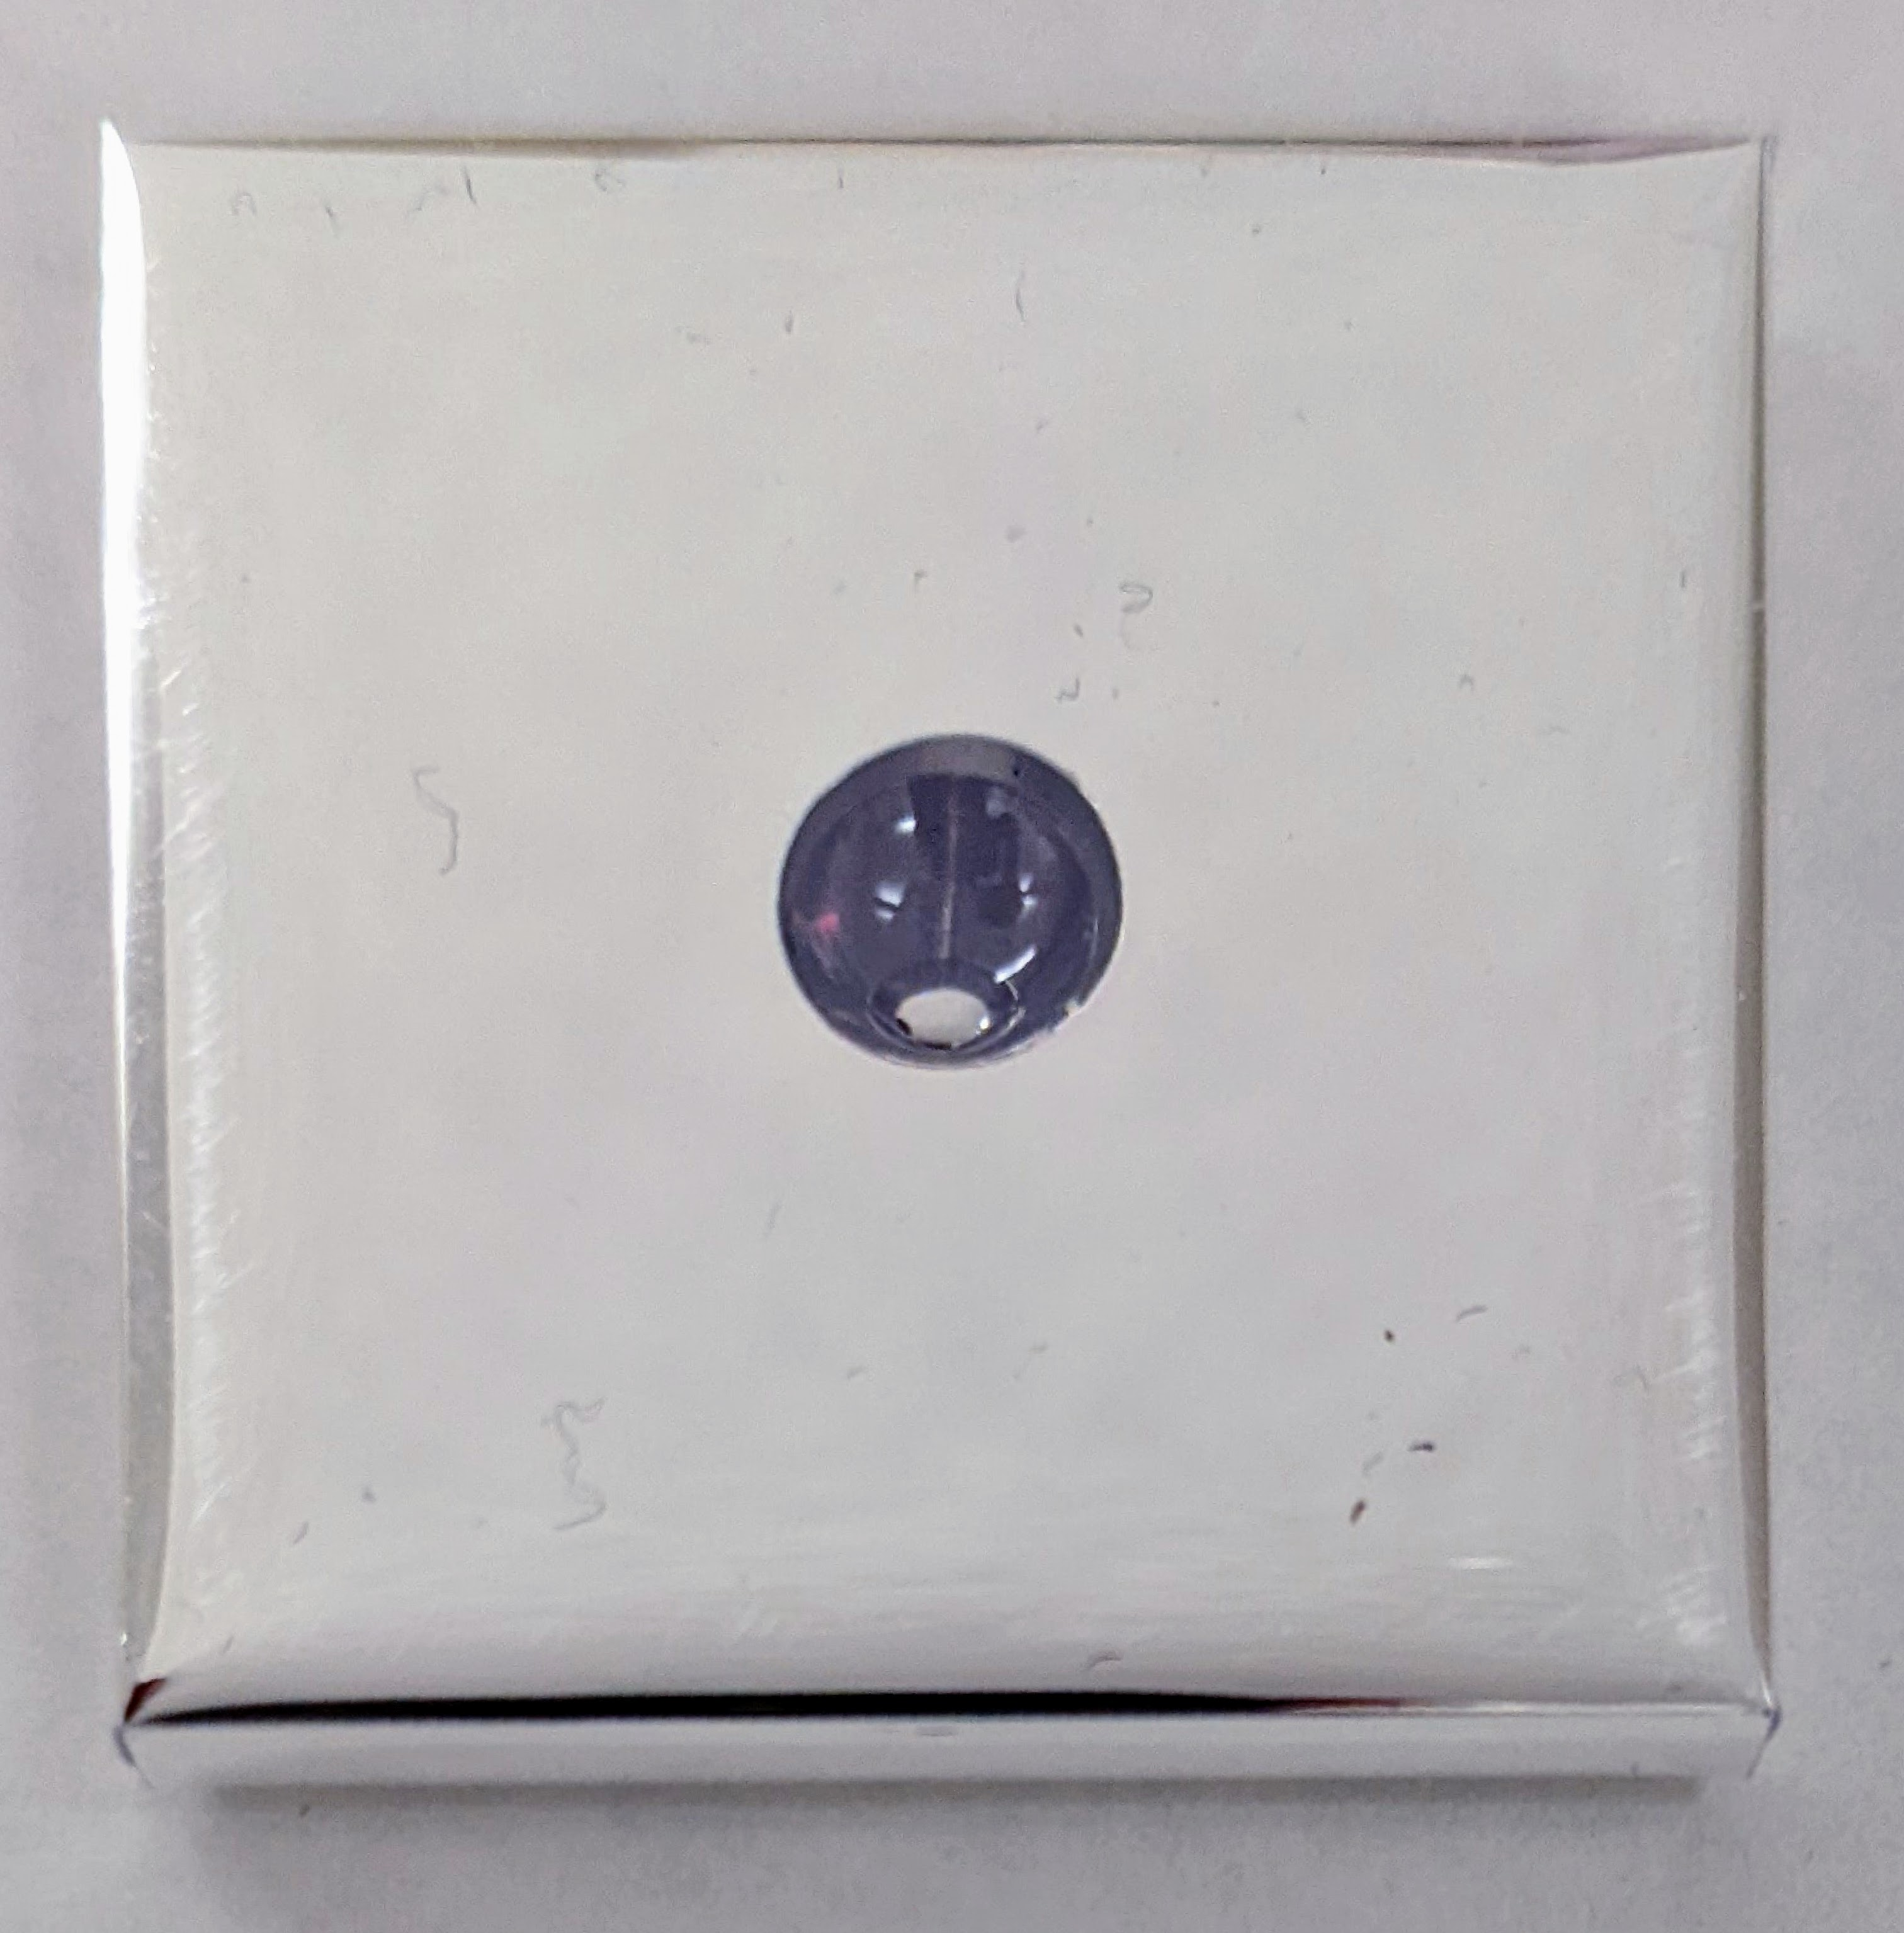
\includegraphics[width=0.4\textwidth]{figures/hgcal/wrapped_tile_down.jpg}
  \caption[R18--19 scintillator tile wrapped in ESR]
  {R18--19 scintillator tile wrapped in ESR\@. Left: Up side of the tile, with
    Kapton sticker holding the flaps. Right: Bottom side with center hole
    over dimple.}%
  \label{fig:hgcal-scintillator-tile-wrapped}
\end{figure}

\clearpage
\section{
  Automated Wrapping of Scintillator Tiles
 }\label{ch_hgcal:wrapping}

As mentioned in Section~\ref{ch_hgcal:scint-tiles}, the number
of wrapped scintillator tiles in \gls{ESR} required for the \gls{HGCAL}
is very large, 100--200 thousand tiles. In addition to large number
of tiles, the tiles will be of different sizes and repeatability
in wrapped tile quality is required for reliable performance
of the detector. Figure~\ref{fig:wrapper-overview-1} and~\ref{fig:wrapper-overview-2}
shows the overview
of automated wrapped being developed at \gls{NICADD}.

\begin{figure}[!ht]
  \centering
  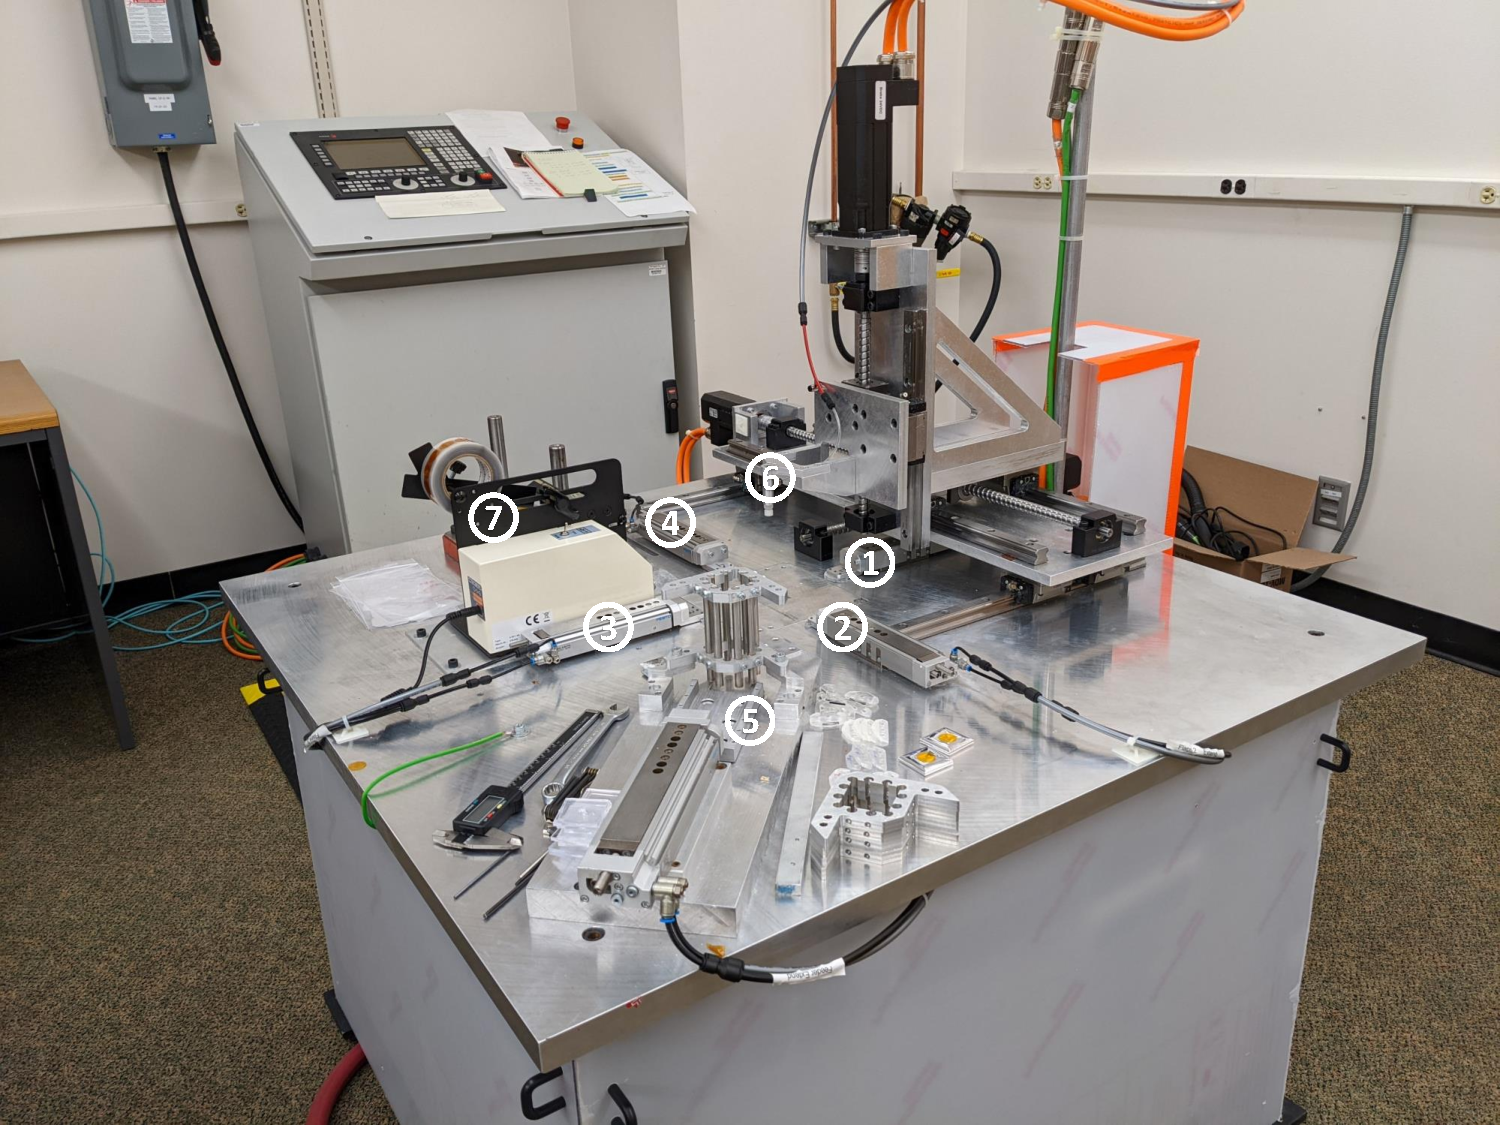
\includegraphics[width=\textwidth,page=1]{figures/wrapper_machine_pics.pdf}
  \caption[Automated scintillator tile wrapper overview]
  {Automated scintillator tile wrapper overview. Shown in picture with labels are,
    1--4: Actuator arms for folding the cut ESR flaps over the tiles,
    5: Tile magazine and dispenser assembly, 6: \textit{z}-axis end-effector
    with vacuum suction, 7: Kapton sticker dispenser.}%
  \label{fig:wrapper-overview-1}
\end{figure}

The machine is built to provide motion in \textit{xyz}-axes
and controlled by G-code programming language.
The second main components of the wrapper are actuators and vacuum
suction, actuator have arm that can extend and retract quickly with the
pressurized air, both pressurized air and vacuum are controlled
by solenoid switch which is programmed the help
of programmable logic controller and can be used in G-code programs.

\begin{figure}[!ht]
  \centering
  \includegraphics[width=\textwidth,page=2]{figures/wrapper_machine_pics.pdf}
  \caption[Tile folding station and ESR magazine]
  {Tile folding station and ESR magazine. Shown in picture
    with labels 1: tile folding station, and 2: ESR magazine.}%
  \label{fig:wrapper-overview-2}
\end{figure}

The final wrapped tile as shown in Figure~\ref{fig:hgcal-scintillator-tile-wrapped}
is done by the machine in following steps:

\begin{itemize}
  \item \textbf{ESR Pickup, and Placement}: \textit{z}-axis end-effector
        picks up the cut \gls{ESR} using vacuum suction from the \gls{ESR} magazine,
        and then places it precisely over the tile pocket in the folding station.
        Placed \gls{ESR} over tile pocket is held into its place with
        the help of vacuum suction, which is built into tile pocket
        seat.
  \item \textbf{Tile Dispenser, Pickup, and Placement}:
        Tiles will be stacked in the magazine at the tile dispenser
        location and an actuator arm will push out a tile
        completely and held in place (right image in Figure~\ref{fig:wrapper-overview-3}) until \textit{z}-axis end-effector
        makes contact and vacuum suction is turned on. Now,
        the actuator arm is retracted and tile is
        picked up and placed over \gls{ESR} at the folding station.
  \item \textbf{ESR Flaps Folding}:
        After \gls{ESR} and tile are placed, and since
        they are held strongly in place with vacuum, the tile pocket
        retracts with the help of actuator connected to it from the bottom.
        At this stage tile is inside pocket and flushed, and \gls{ESR}
        flaps are out and vertical.
        Now the four actuator arms as shown in Figure~\ref{fig:wrapper-overview-4}
        extends and closes \gls{ESR} flaps.
  \item \textbf{Sticker Application}:
        Now the folding actuator arms stay in place until sticker is
        applied using \textit{z}-axis end-effector which
        picks up the sticker from sticker dispenser (left image Figure~\ref{fig:wrapper-overview-3}) and applies it on
        the center of the tile where all flaps corners meet.
  \item \textbf{Wrapped Tile}:
        Final step in wrapping is retracting folding actuator arms,
        pushing out the tile and turning of the vacuum suction of tile pocket.
        Now \textit{z}-axis end-effector picks up the wrapped tile and
        drops into the collection basket.
        Wrapped tile in Figure~\ref{fig:hgcal-scintillator-tile-wrapped}
        is wrapped automatically with this machine.
\end{itemize}

\begin{figure}[!ht]
  \centering
  \includegraphics[width=0.49\textwidth,page=3]{figures/wrapper_machine_pics.pdf}
  \includegraphics[width=0.49\textwidth,page=4]{figures/wrapper_machine_pics.pdf}
  \caption[Sticker and tile dispenser.]
  {Sticker and tile dispenser, Left: Sticker dispenser
    with kapton tape roll. Right: Tile dispenser with tile magazine.}%
  \label{fig:wrapper-overview-3}
\end{figure}

\begin{figure}[!ht]
  \centering
  \includegraphics[width=0.49\textwidth,page=6]{figures/wrapper_machine_pics.pdf}
  \includegraphics[width=0.49\textwidth,page=7]{figures/wrapper_machine_pics.pdf}
  \caption[Tile folding station]
  {Tile folding station. Left: Flushed tile pocket at the center
    and retracted actuator arms. Right: After all the
    arms are extended during wrapping.}%
  \label{fig:wrapper-overview-4}
\end{figure}

\clearpage
\section{
  Signal-to-Noise Ratio
 }

As discussed earlier in the Section~\ref{ch_hgcal:technical-design},
for \gls{HGCAL} to retain its precision till the end-of-life it needs
good \gls{SNR}, which is defined as \gls{SNR} \( > 3\). In this section we
will discuss formulation and input to the calculation of \gls{SNR}, and
the results of optimal configuration by minimizing cost and
retaining good \gls{SNR}.

\subsection{
  Formulation
}

\gls{MIP} Signal-to-Noise ratio for the scintillator tile coupled directly
with SiPM is formulated as~\cite{cms-dn-17-001}:

\begin{equation}
  \frac{S}{N} =
  \frac{
  (\texttt{MIP}^{*})
  \sqrt{\frac{A_{t,\texttt{ref}}}{A_{t}}}
  \left(\frac{A_{s}}{A_{s,\texttt{ref}}}\right)
  (\texttt{Radiation Loss})
  }
  {
  (\texttt{SiPM}_\texttt{noise,base})
  \sqrt{\frac{A_{s}}{A_{s,\texttt{base}}}}
  \sqrt{1.88^{\frac{T_{s}-T_{s,\texttt{base}}}{10^{\circ} \text{ C}}}}
  \sqrt{\frac{f}{f_{\texttt{base}}}}
  }
\end{equation}

where,

\begin{itemize}
  \item \( \texttt{MIP}^{*} \): is the \gls{MIP} measurement of the
        scintillator tile with a scale factor to account for \gls{SiPM} device
        \gls{PDE} difference used during testbeam measurement and
        \gls{SiPM} expected to be used.
  \item \( A_t \): is the area of the tile for which the \gls{SNR} is being
        evaluated and subscript \( \texttt{ref} \) means the area of tile
        corresponding to \gls{MIP} measurement.
  \item \( A_s \): similar to \( A_t \), it is instead the area of the
        \gls{SiPM} device coupled to scintillator tile.
  \item \( \texttt{Radiation Loss} \): is the loss in light output
        due to the radiation dose received, it is expressed as:
        \begin{gather}
          e^{-R/D_{c}} \\
          D_c = (6.0 \text{ Mrad})
          {\left( \frac{R}{1 \xspace\text{ krad/hr}} \right)}^{0.35}
        \end{gather}
        where \( R \) is the dose rate in \( \text{krad/hr} \), and \( D_c \) is the
        dose constant, and both are obtained from \textsc{FLUKA} simulations.
  \item \( \texttt{SiPM}_\texttt{noise,base} \):
        is the \gls{RMS} value in \gls{PE} of
        signal noise received from \gls{SiPM} from thermal excitation
        of electrons in pixels, also called \gls{DCR}.
        In addition to thermal effects, irradiation of silicon
        also increases this noise. \( \texttt{base} \)
        in the subscript refers to \gls{DCR} measurement conditions such as
        temperature of the \gls{SiPM} \( T_{s,\texttt{base}}\),
        area of \gls{SiPM} \( A_{s,\texttt{base}}\) and fluence \( f_{\texttt{base}}\).
  \item \( T_s \): is the temperature of the \gls{HGCAL} hence the \gls{SiPM}
        at which it will be operated, which is \( -30^\circ \text{ C} \).
  \item \( f \): is the amount of fluence \gls{SiPM} will receive over its
        lifetime of operation in \gls{HGCAL} i.e.~after 3000 \fbinv{}.
\end{itemize}

\subsection{
  Testbeam and SiPM Noise Inputs
}

\gls{FNAL} conducted testbeam measurement in January 2020 on both cast and injection
molded scintillator tiles wrapped in \gls{ESR} with \gls{SiPM}
using \gls{FNAL} 120 \GeV{} testbeam facility. The scintillator tiles
used in testbeam were of dimensions \( 30 \times 30 \mm{}^{2} \) square tiles,
and \gls{SiPM} device used was Hamamatsu S13360--1350CS (\( 1.3 \times 1.3 \mm{}^{2} \))
~\cite{mppc-13360,testbeam-fnal-2020}.

The \gls{MIP} measured from testbeam are 35 \gls{PE} for cast scintillator tiles,
and 25 \gls{PE} for injection molded with \gls{SiPM} operated at
voltage of 54.26 V, which is \gls{OV} of 2.5V (I-V method) (equivalent
to 3.0V when measured with gain method).
Currently \gls{SiPM} device class expected to used in \gls{HGCAL}
is Hamamatsu S14160 with 15\micron{} pixel size (dubbed as HDR15)
and \(2, 4, 9 \mm{}^{2} \) in
area operated at \gls{OV} of 2V (I-V method),
using ratio of \glspl{PDE} of these devices
we can calculate PDE scale factor as,

\begin{equation}
  = \frac{\text{PDE of S14160 at } V_O = 2V}
  {\text{PDE of S13360 at } V_O = 3V}
  = \frac{34.9}{40}
  = 0.8725
\end{equation}

this gives, \( \texttt{MIP}^{*} \) value to be 30.5 \gls{PE} for cast
and 21.8 \gls{PE} for injection molded scintillator tiles.

\gls{DCR} measurement for HDR15 (\( 2 \mm{}^2 \)) \glspl{SiPM}
irradiated to \( 5 \times {10}^{13} \text{ n}/\cm{}^2 \)
operated at \gls{OV} = 2V (I-V method) and at temperature \( -30^{\circ} \text{ C}\)
is equivalent to \gls{RMS} value of 19 \gls{PE} with 15 \nanoseconds{} integration time
period.

Using the testbeam measurement of scintillator tiles, and irradiated \gls{SiPM}
\gls{DCR} measurement end-of-life scenario estimation of
detector performance was done for combinations
of types of scintillator tiles and different area of HDR15 \glspl{SiPM}.

\subsection{
  Scenarios
}

Five combinations of scintillator material and \gls{SiPM} active area
were considered in two different scenarios as:

\begin{itemize}
  \item \textbf{Scene A}: In this scene, \glspl{SiPM} with larger active area
        are preferred, followed by injection molded over cast scintillator.
        \begin{enumerate}
          \item Injection Molded Scintillator Tiles and SiPM of active area \( 2\mm{}^2 \).
          \item Injection Molded Scintillator Tiles and SiPM of active area \( 4\mm{}^2 \).
          \item Cast Scintillator Tiles and SiPM of active area \( 2\mm{}^2 \).
          \item Cast Scintillator Tiles and SiPM of active area \( 4\mm{}^2 \).
          \item Cast Scintillator Tiles and SiPM of active area \( 9\mm{}^2 \).
        \end{enumerate}
  \item \textbf{Scene B}: In this scene, brighter scintillator
        i.e.~cast over injection is preferred, followed by
        increasing size of \glspl{SiPM}.
        \begin{enumerate}
          \item Injection Molded Scintillator Tiles and SiPM of active area \( 2\mm{}^2 \).
          \item Cast Scintillator Tiles and SiPM of active area \( 2\mm{}^2 \).
          \item Injection Molded Scintillator Tiles and SiPM of active area \( 4\mm{}^2 \).
          \item Cast Scintillator Tiles and SiPM of active area \( 4\mm{}^2 \).
          \item Cast Scintillator Tiles and SiPM of active area \( 9\mm{}^2 \).
        \end{enumerate}
\end{itemize}

Individual's \gls{SNR} of each combination when used alone is shown in
Figure~\ref{fig:hgcal-scint-everywhere} after 3000 \fbinv{}.
Clearly injection molded scintillator cannot be used in leftmost layers,
and even with cast scintillator it is possible only when using
\gls{SiPM} with large active area.

\begin{figure}
  \centering
  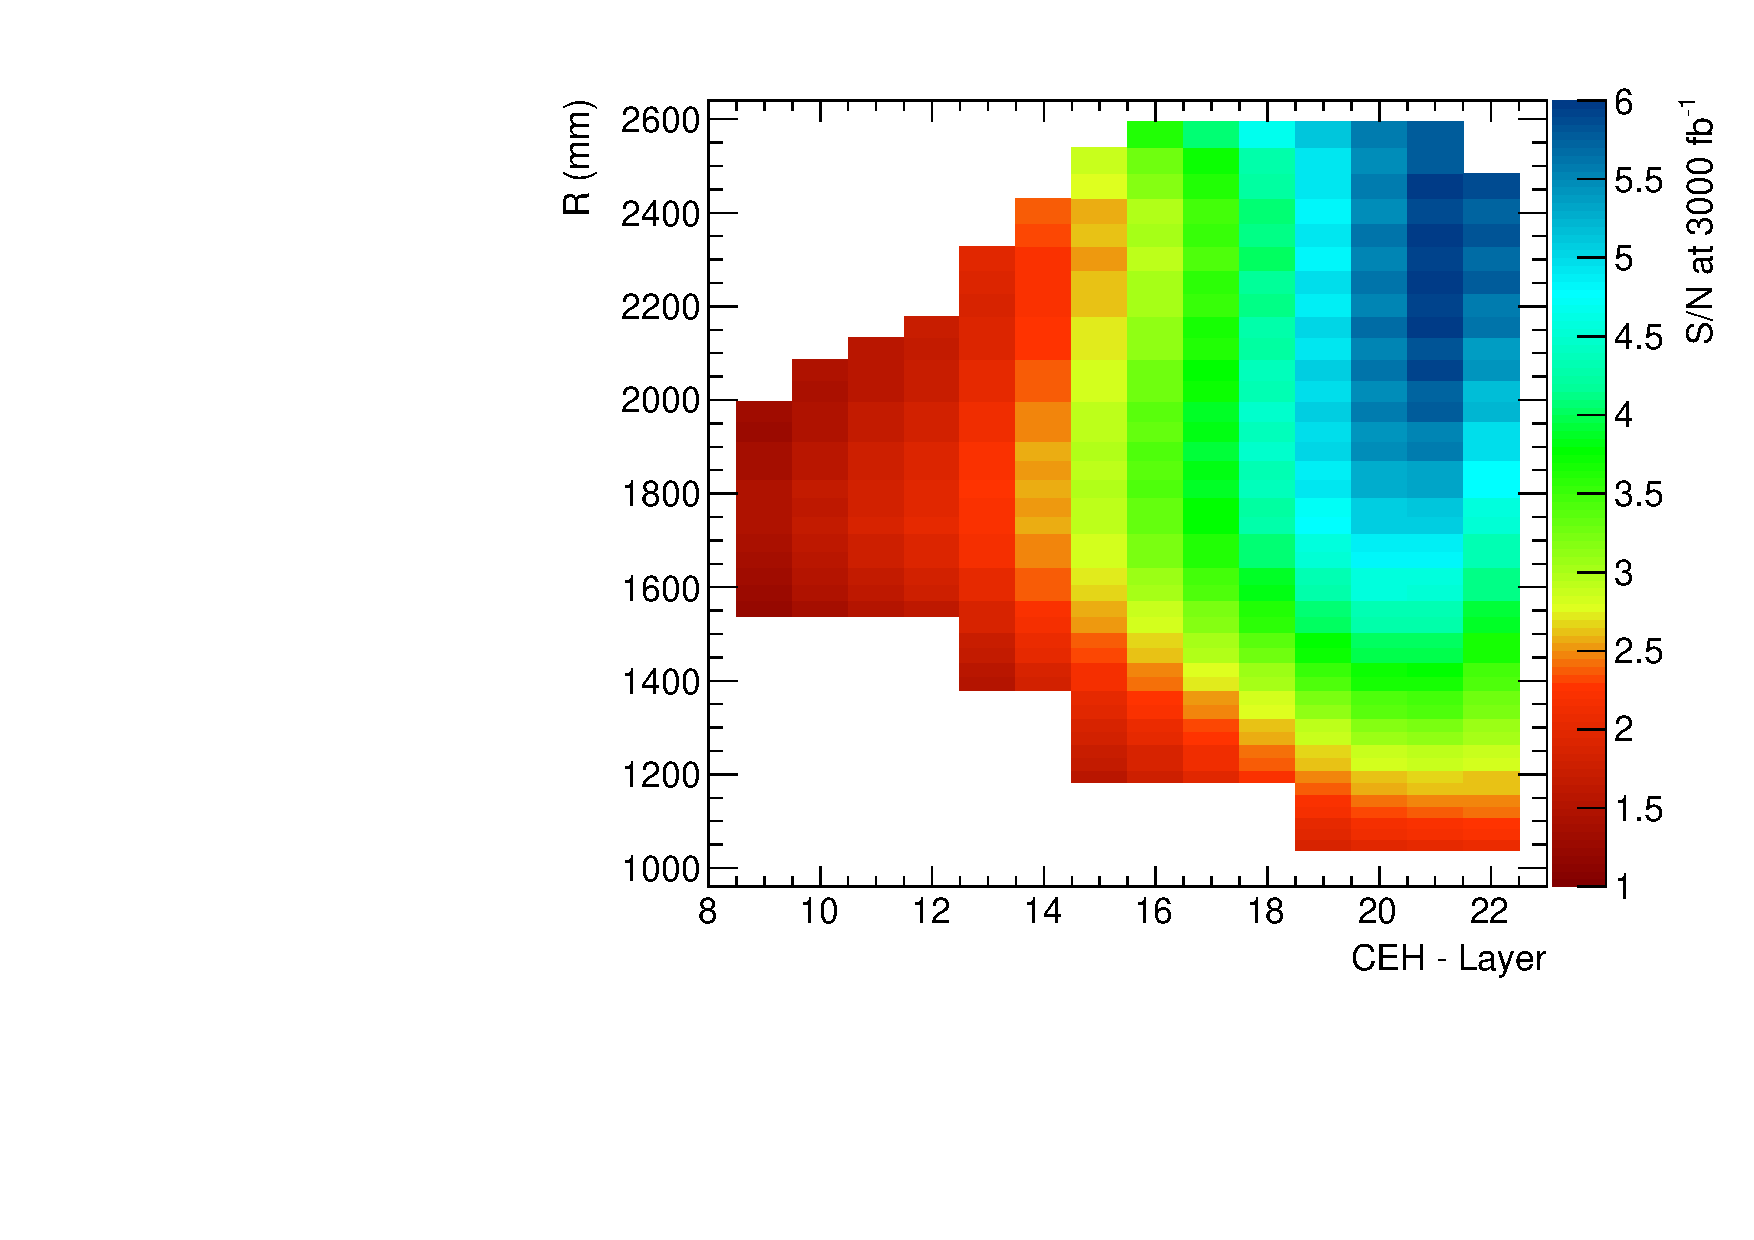
\includegraphics[width=0.45\textwidth]{figures/hgcal/plot_zr/mold_mip_25_pdeC_34.9_40_sipmA_2.0_rad_4_sipmN_52_sipmAC_default_tileAC_default_S_N.pdf}\\
  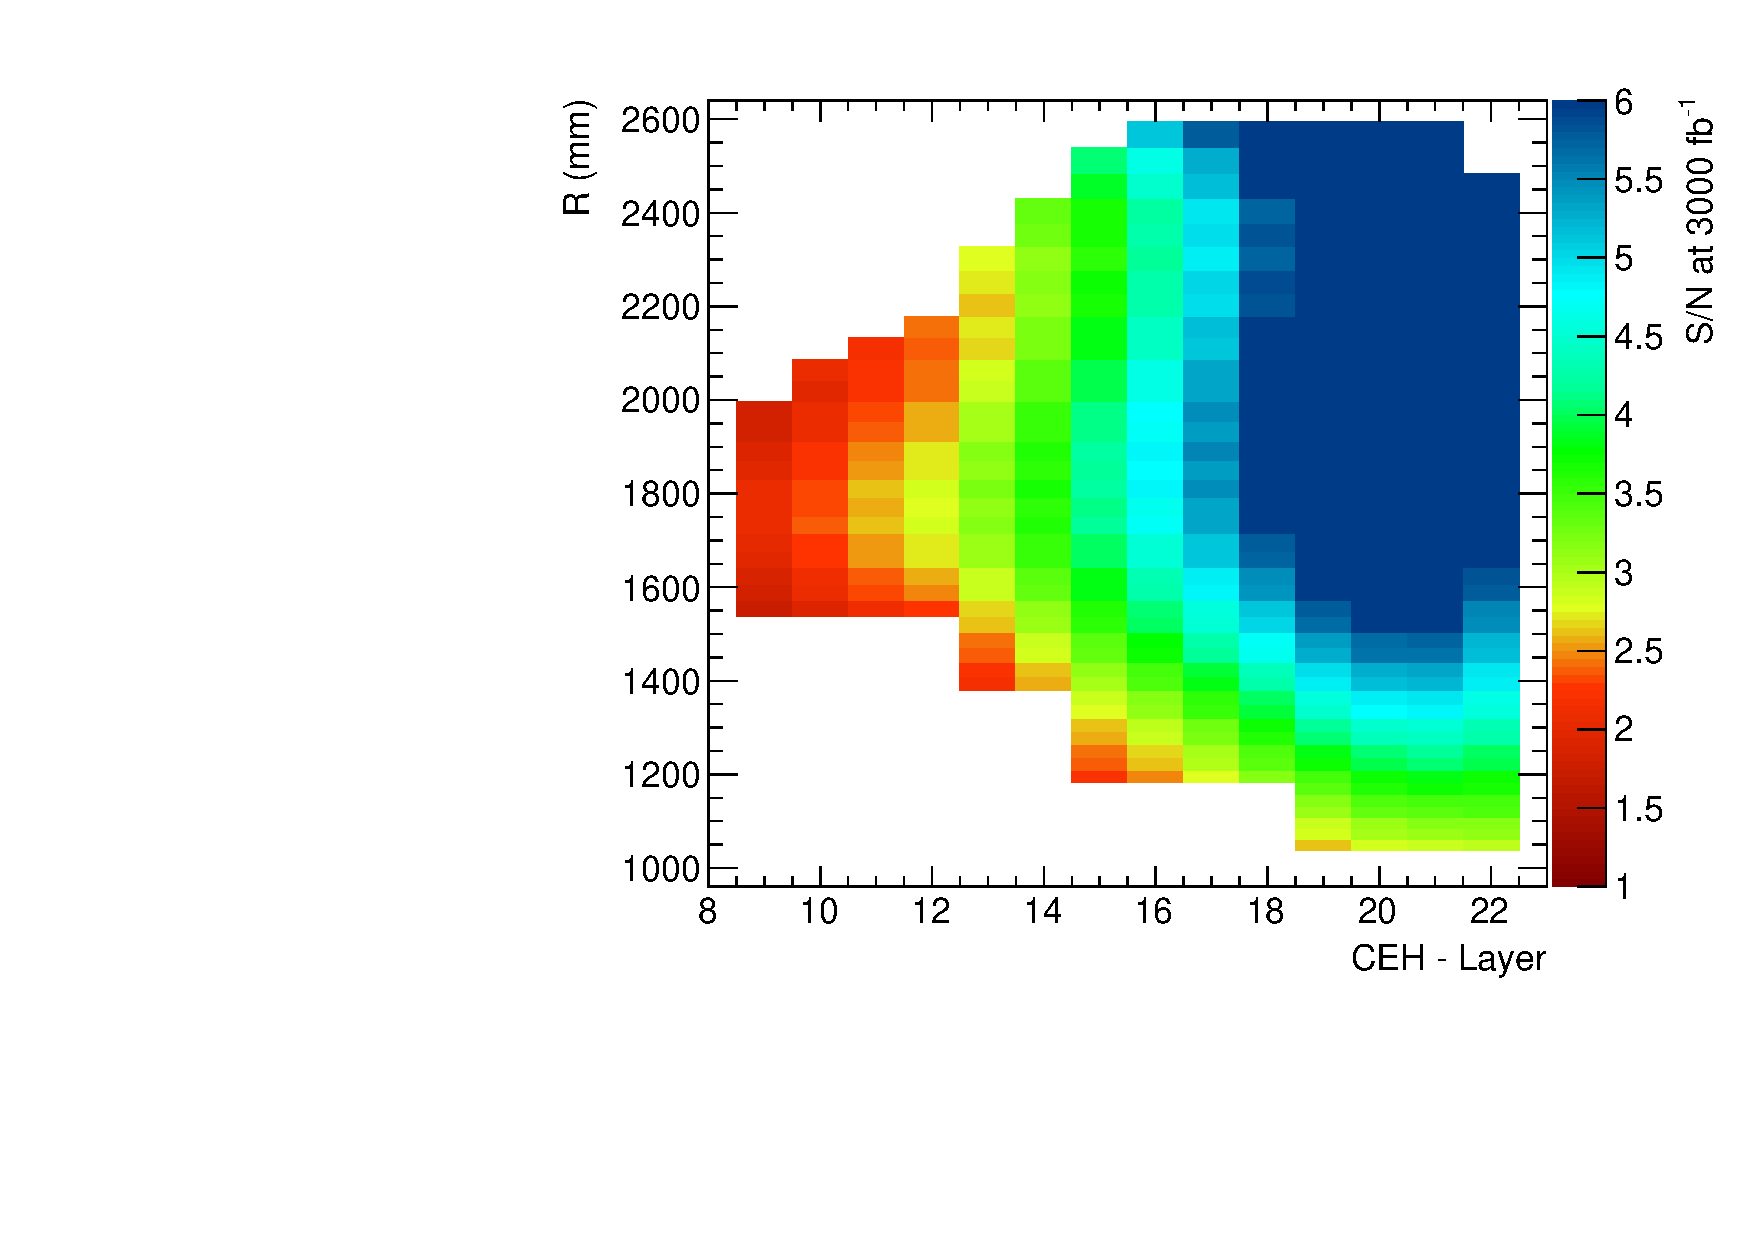
\includegraphics[width=0.45\textwidth]{figures/hgcal/plot_zr/mold_mip_25_pdeC_34.9_40_sipmA_4.0_rad_4_sipmN_52_sipmAC_default_tileAC_default_S_N.pdf}
  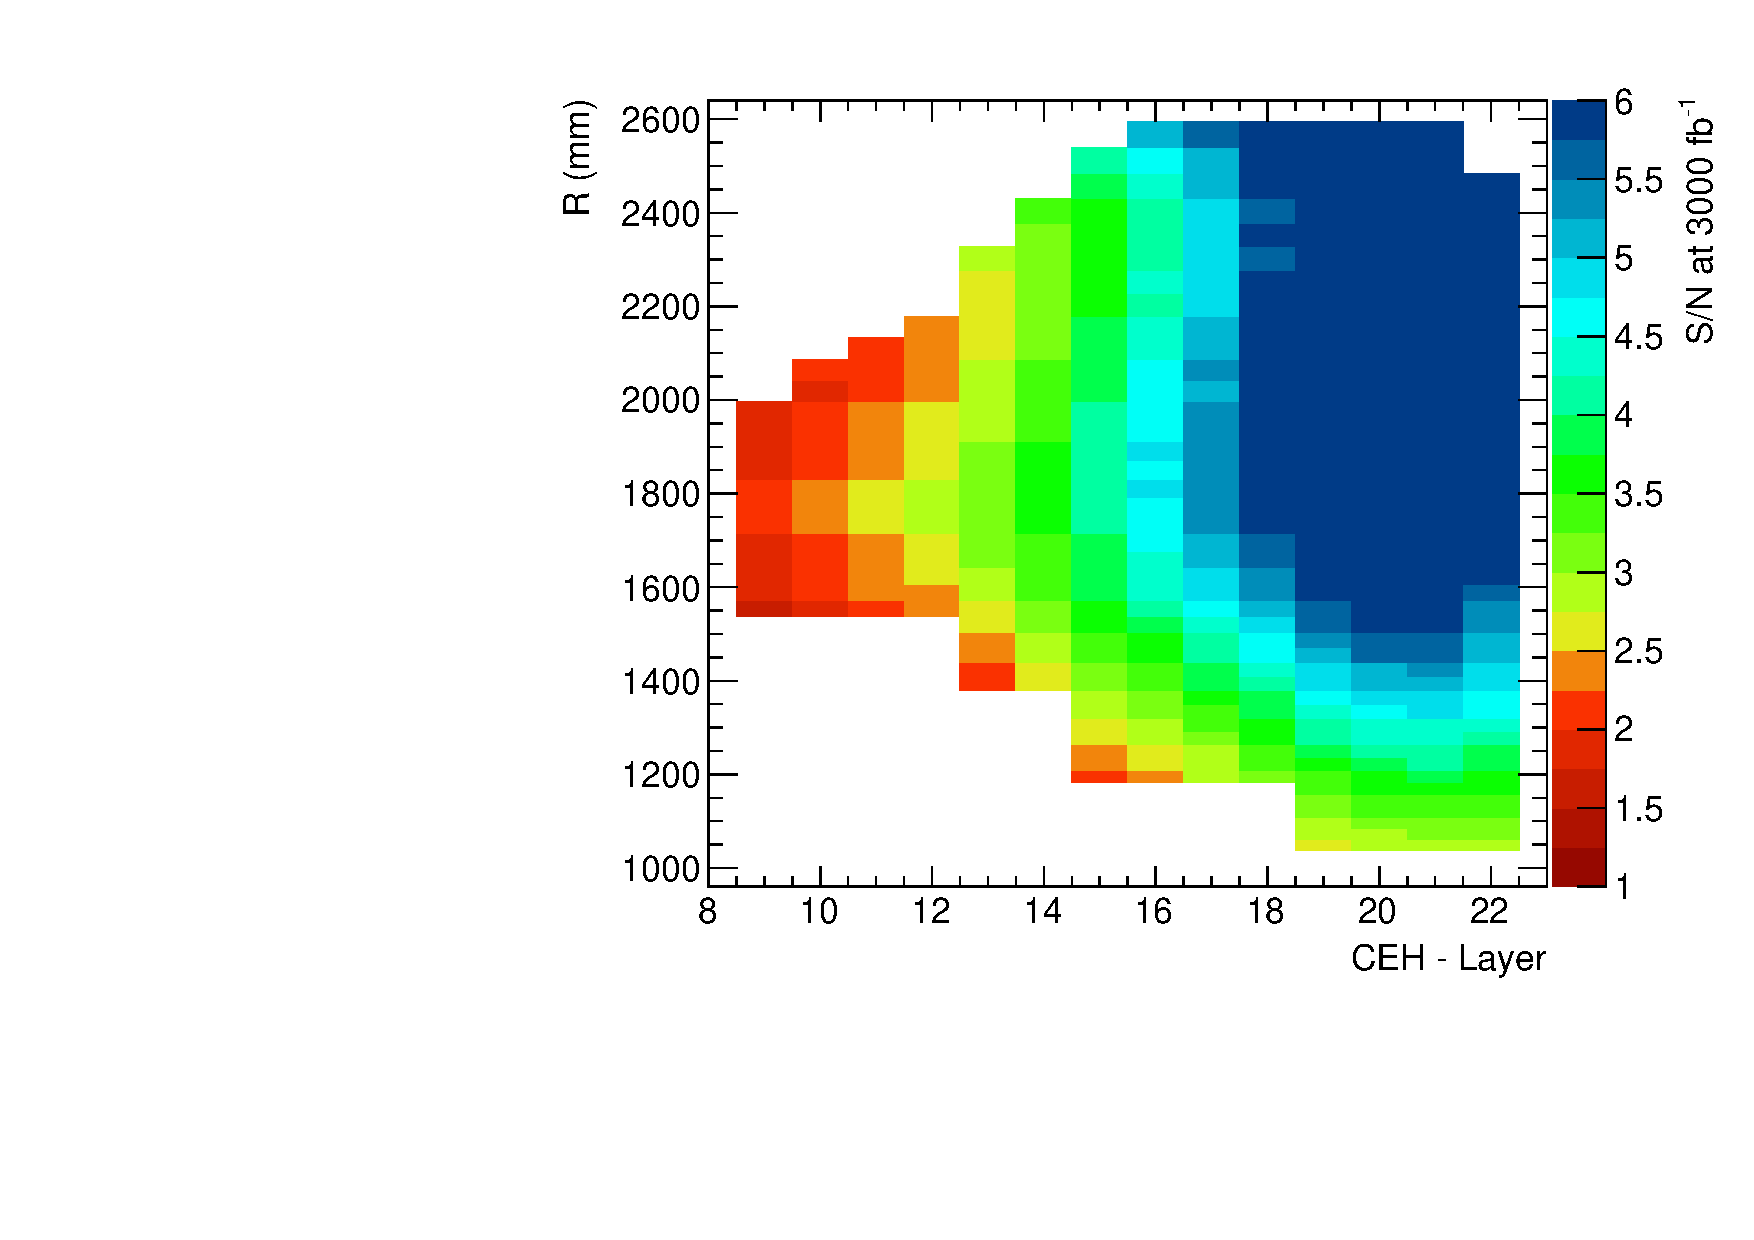
\includegraphics[width=0.45\textwidth]{figures/hgcal/plot_zr/cast_mip_35_pdeC_34.9_40_sipmA_2.0_rad_4_sipmN_52_sipmAC_default_tileAC_default_S_N.pdf}\\
  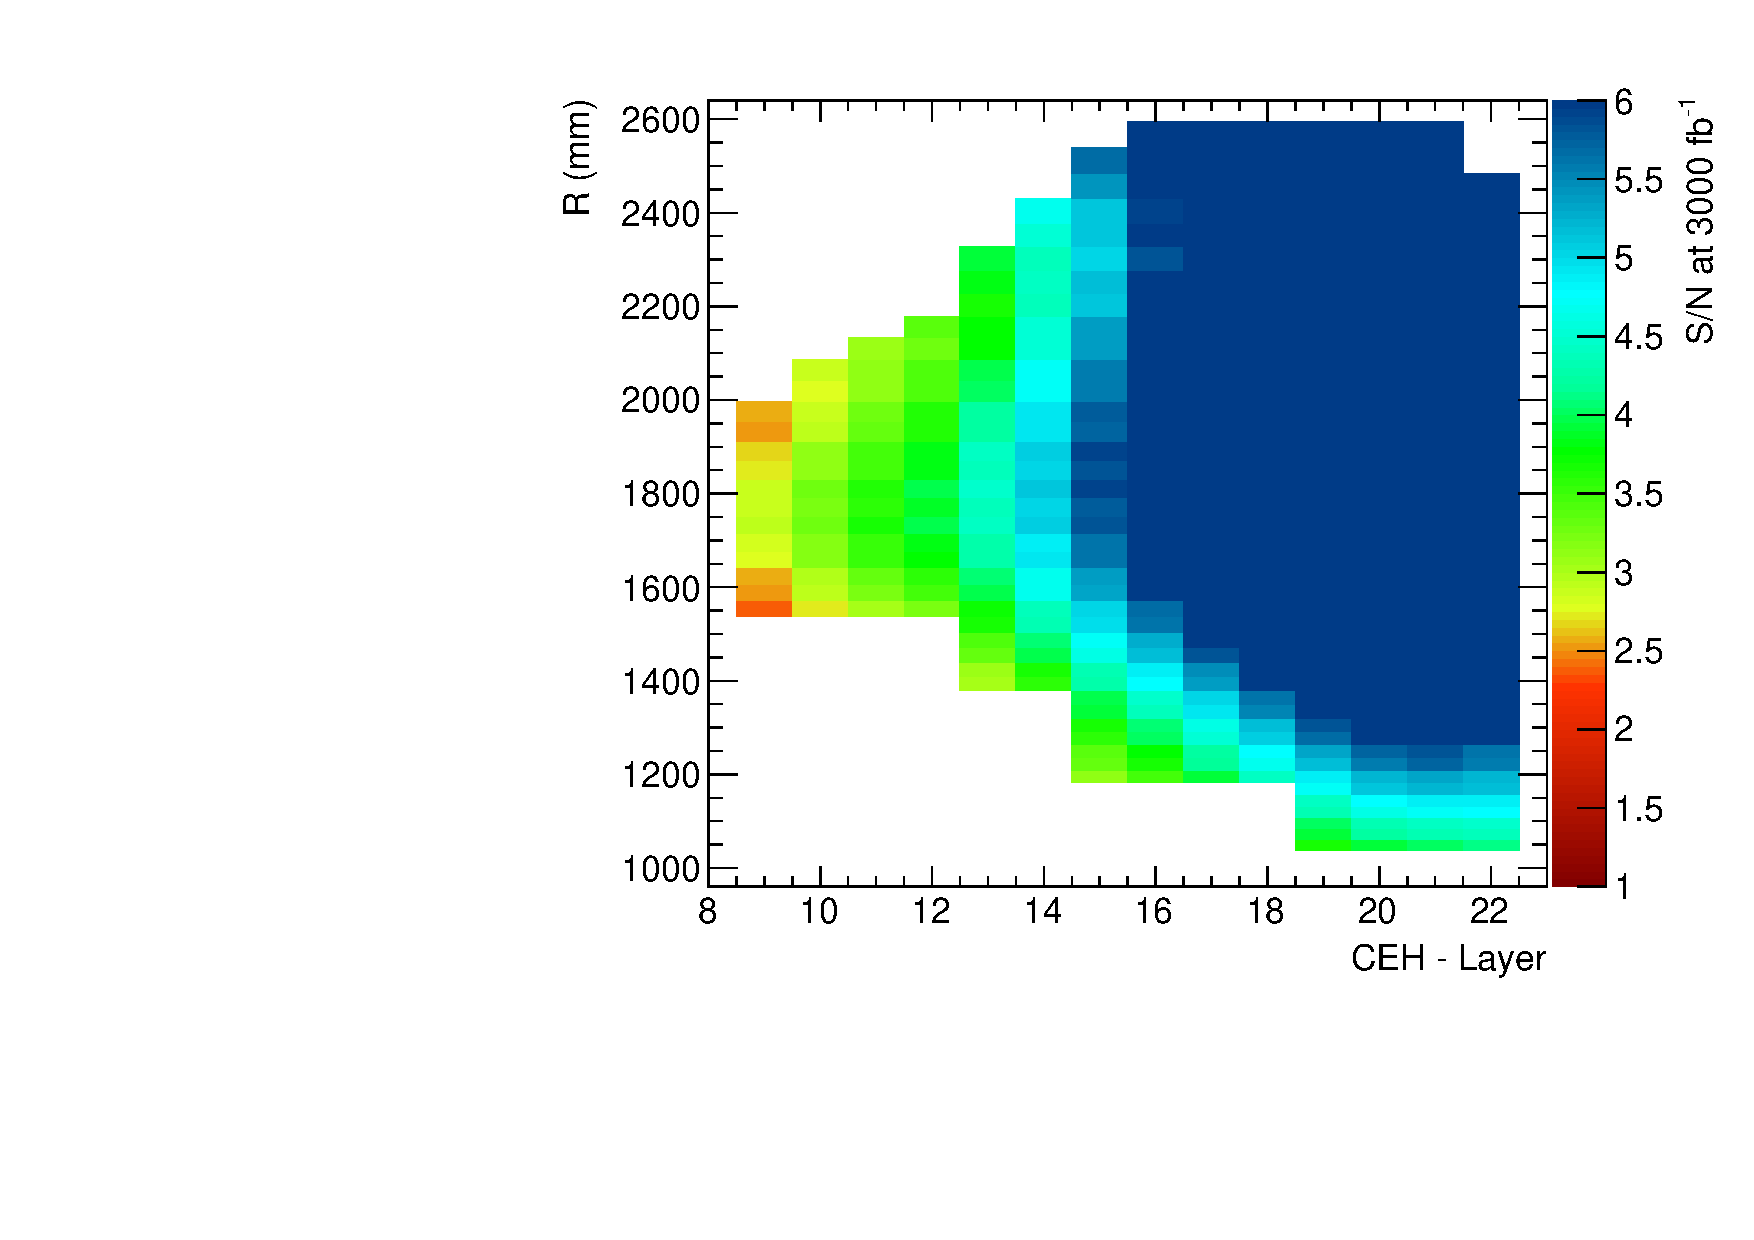
\includegraphics[width=0.45\textwidth]{figures/hgcal/plot_zr/cast_mip_35_pdeC_34.9_40_sipmA_4.0_rad_4_sipmN_52_sipmAC_default_tileAC_default_S_N.pdf}
  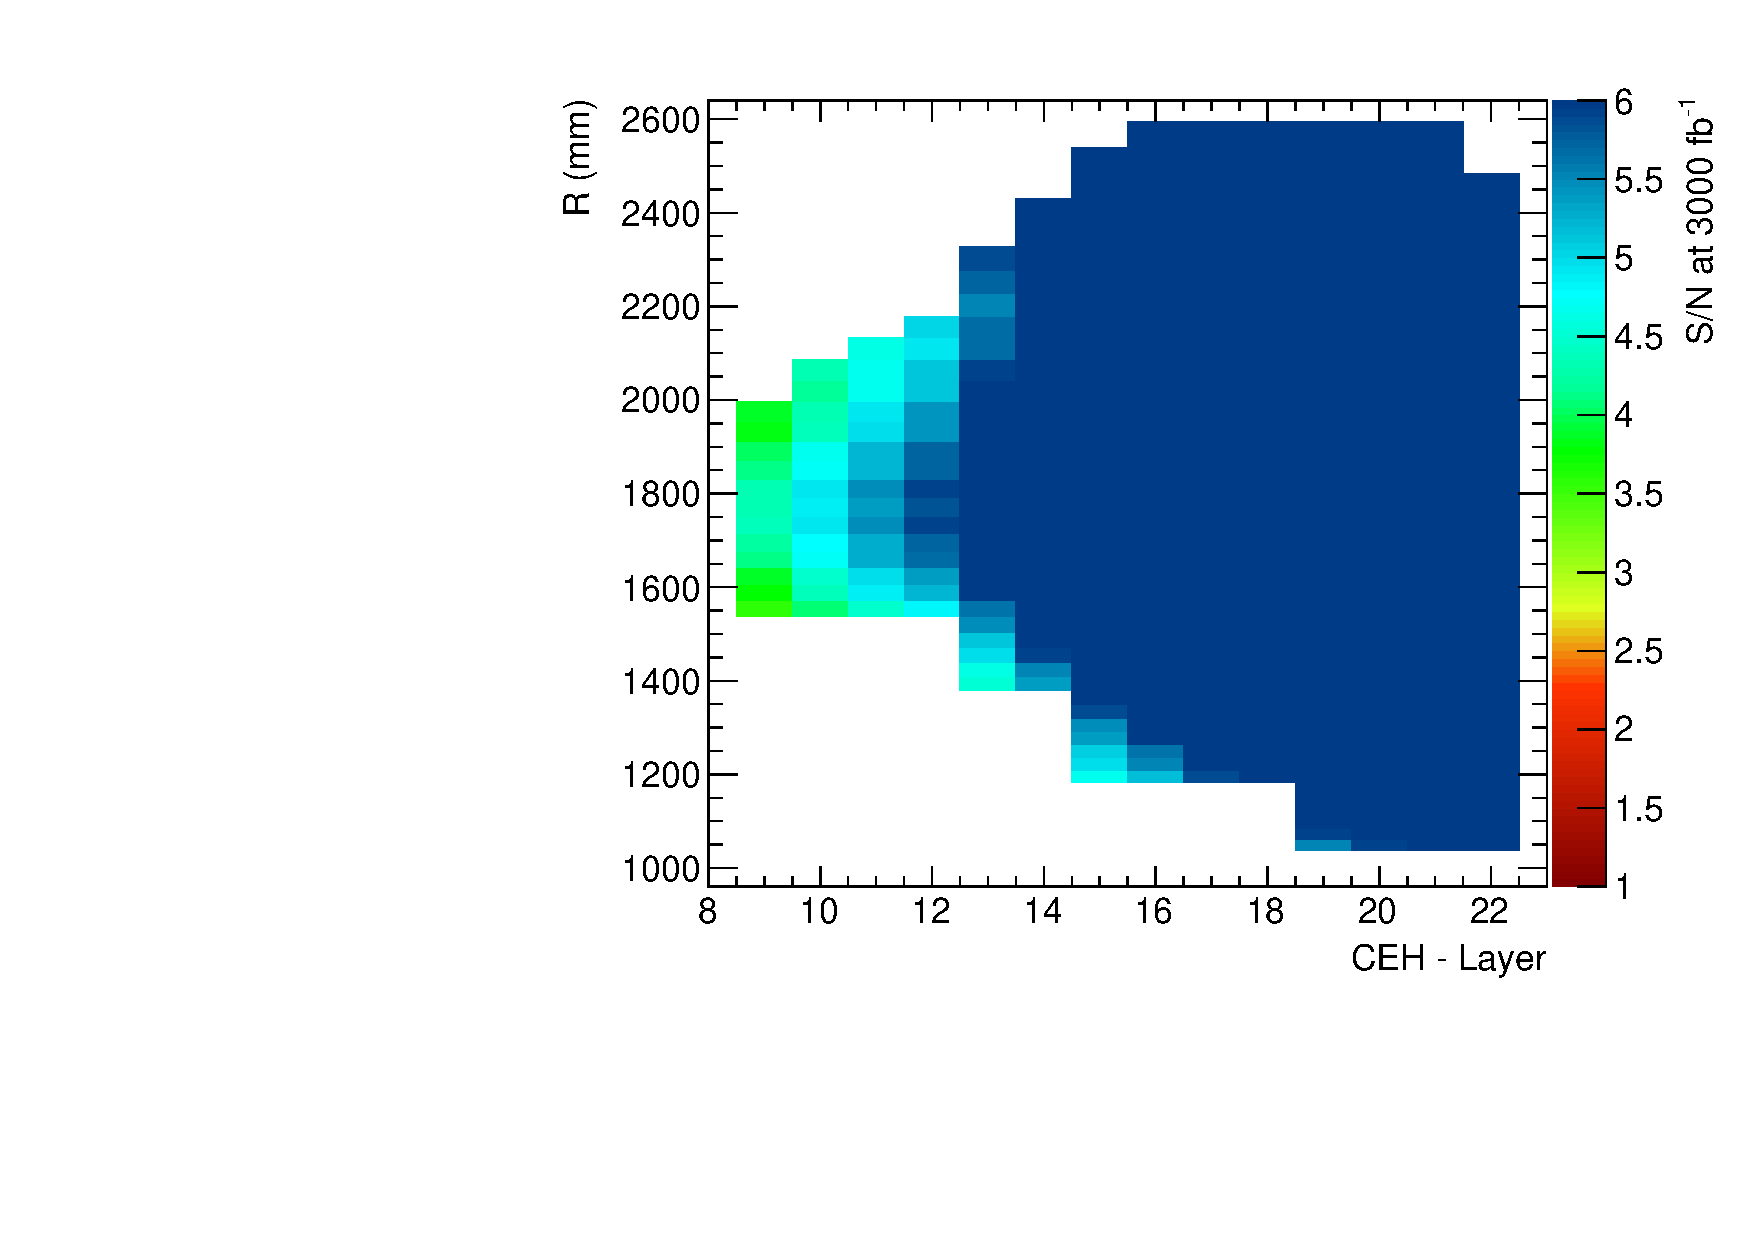
\includegraphics[width=0.45\textwidth]{figures/hgcal/plot_zr/cast_mip_35_pdeC_34.9_40_sipmA_9.0_rad_4_sipmN_52_sipmAC_default_tileAC_default_S_N.pdf}
  \caption[Scintillator performance with various active area size
    of \gls{SiPM}]{Scintillator performance with various active area size
    of \gls{SiPM}. Top row from Left to Right: Injection Molded
    Scintillator with \gls{SiPM} \( 2 \) and \( 4\mm{}^2 \) active area device.
    Bottom row from Left to Right: Cast Scintillator with
    \gls{SiPM} \( 2,4 \) and \( 9\mm{}^2 \) active area device.}%
  \label{fig:hgcal-scint-everywhere}
\end{figure}

\subsection{
  Results and Conclusion
}

Since for assembly of scintillator tiles on tileboard, it is preferred
to have single type of scintillator with \gls{SiPM} combination.
For this reason, each scene is evaluated in the preference order
and tileboard is assigned a combination only
if all the rings in it are able to satisfy \gls{SNR} \( > 3\).
Figure~\ref{fig:hgcal-scenes-fnal-jan20} shows final
results of how both scenes fill tileboards in \gls{CE-H}.

\begin{figure}[!ht]
  \centering
  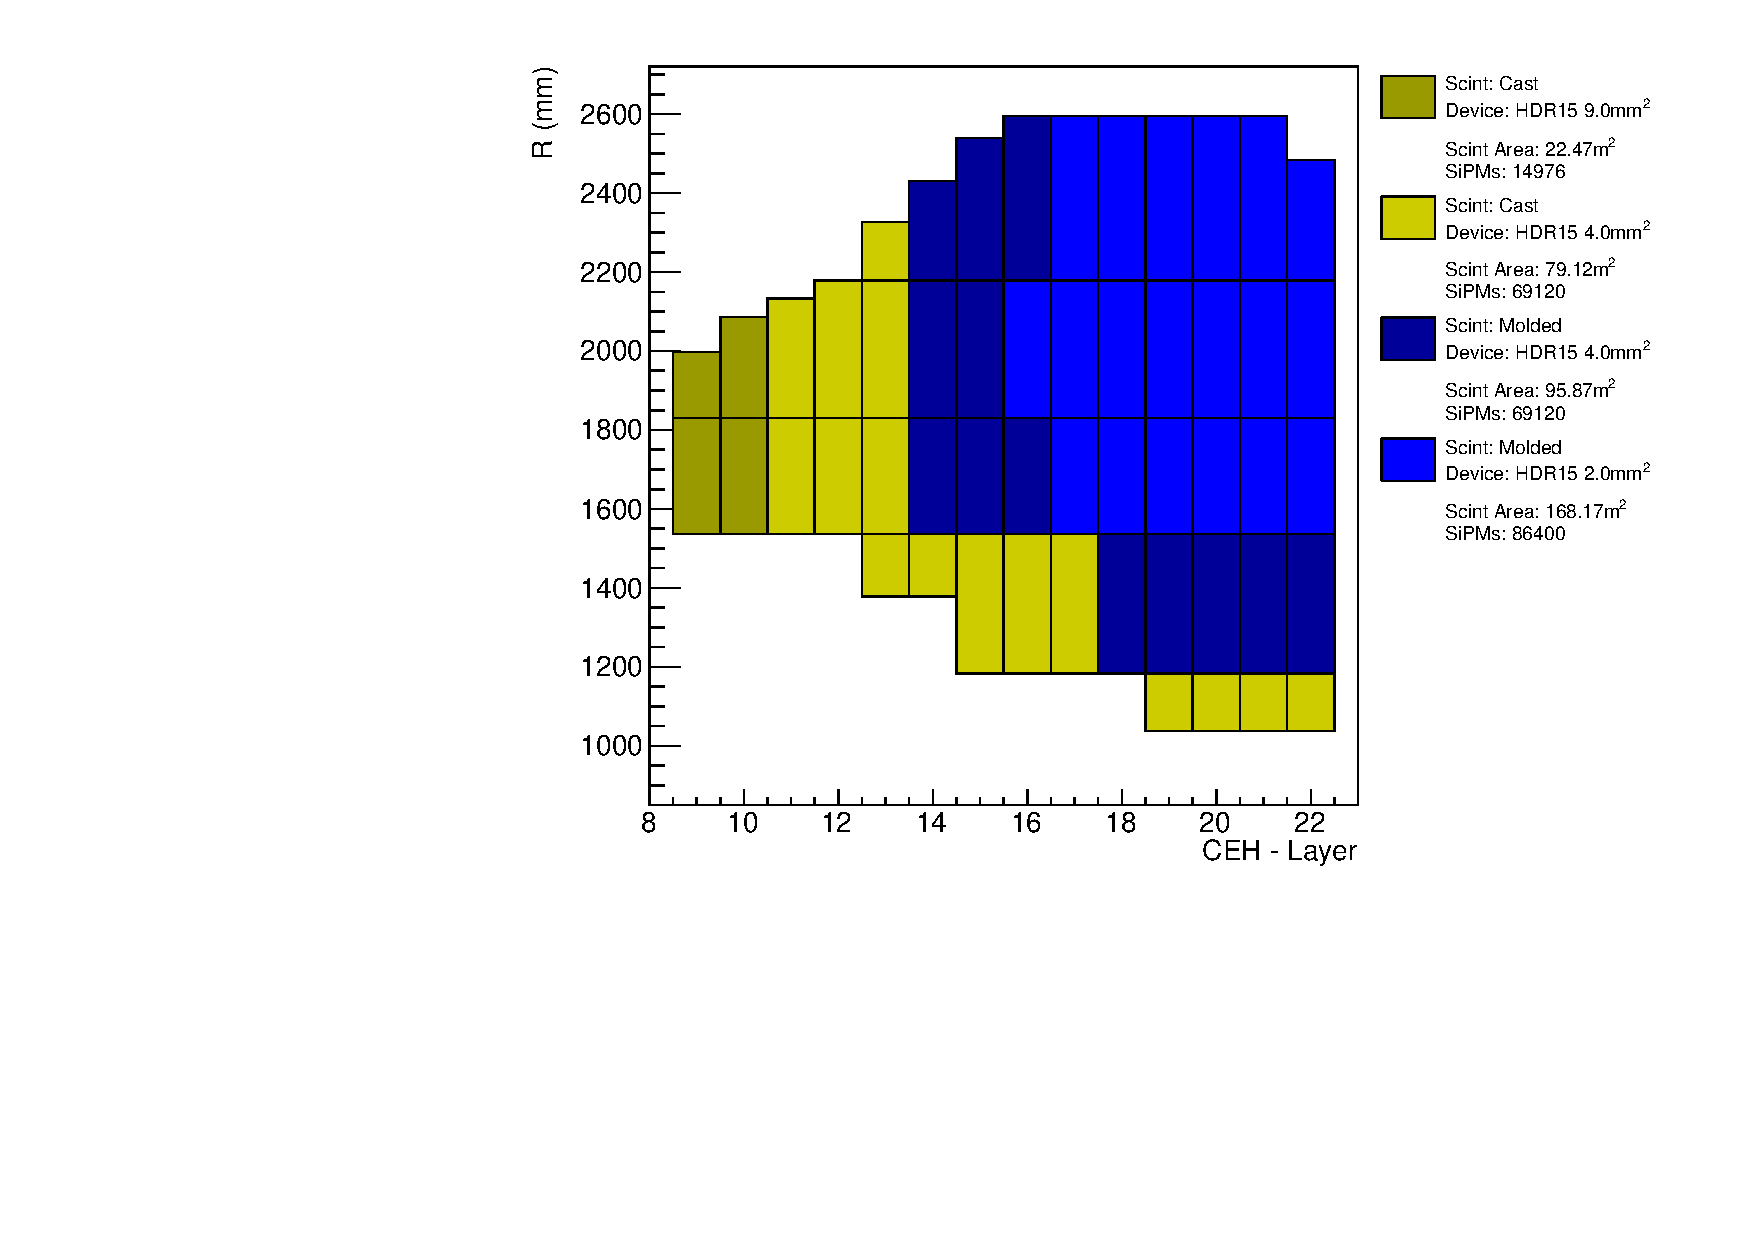
\includegraphics[trim={400 370 20 10},clip,width=0.24\textwidth]{figures/hgcal/plot_scenes/sceneA_jan20_fix_vto2p0_with9mm2.pdf}
  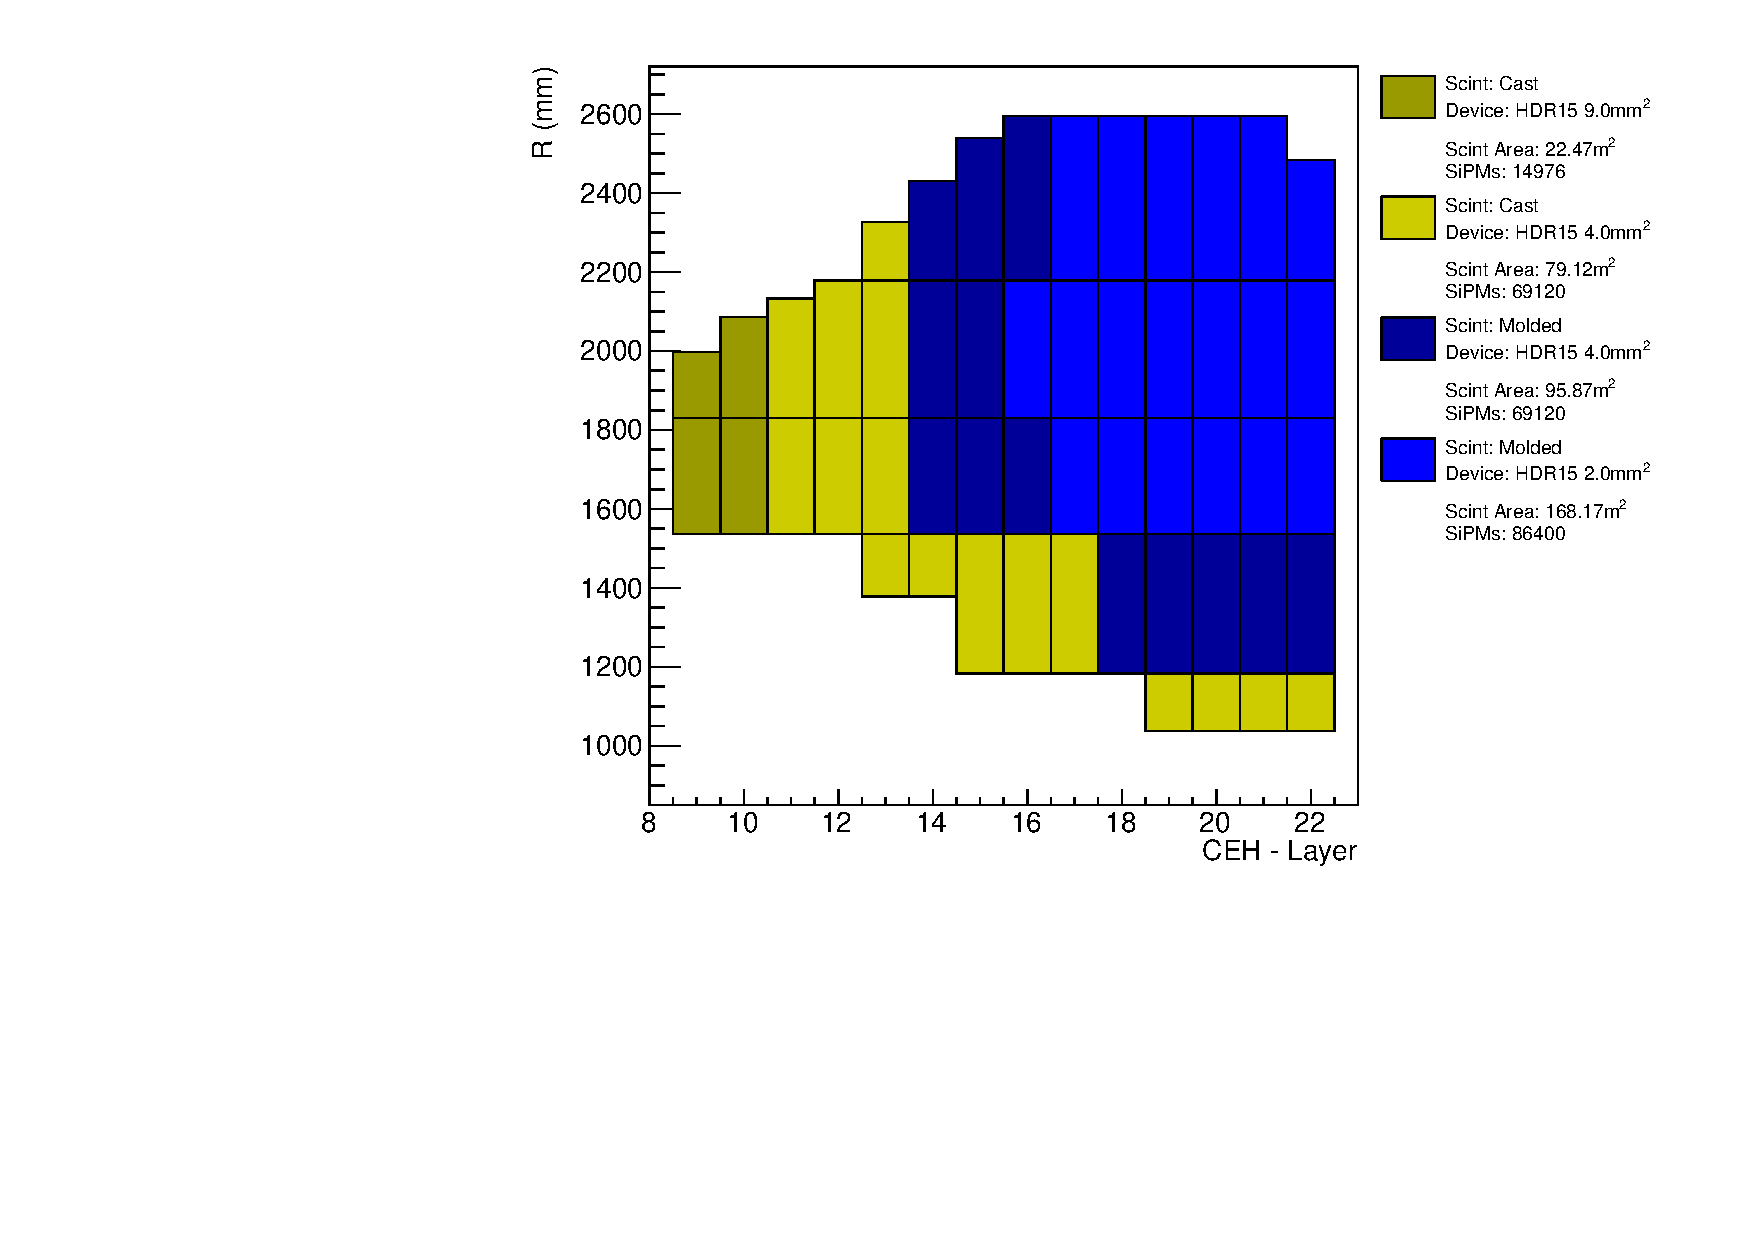
\includegraphics[trim={400 310 20 70},clip,width=0.24\textwidth]{figures/hgcal/plot_scenes/sceneA_jan20_fix_vto2p0_with9mm2.pdf}
  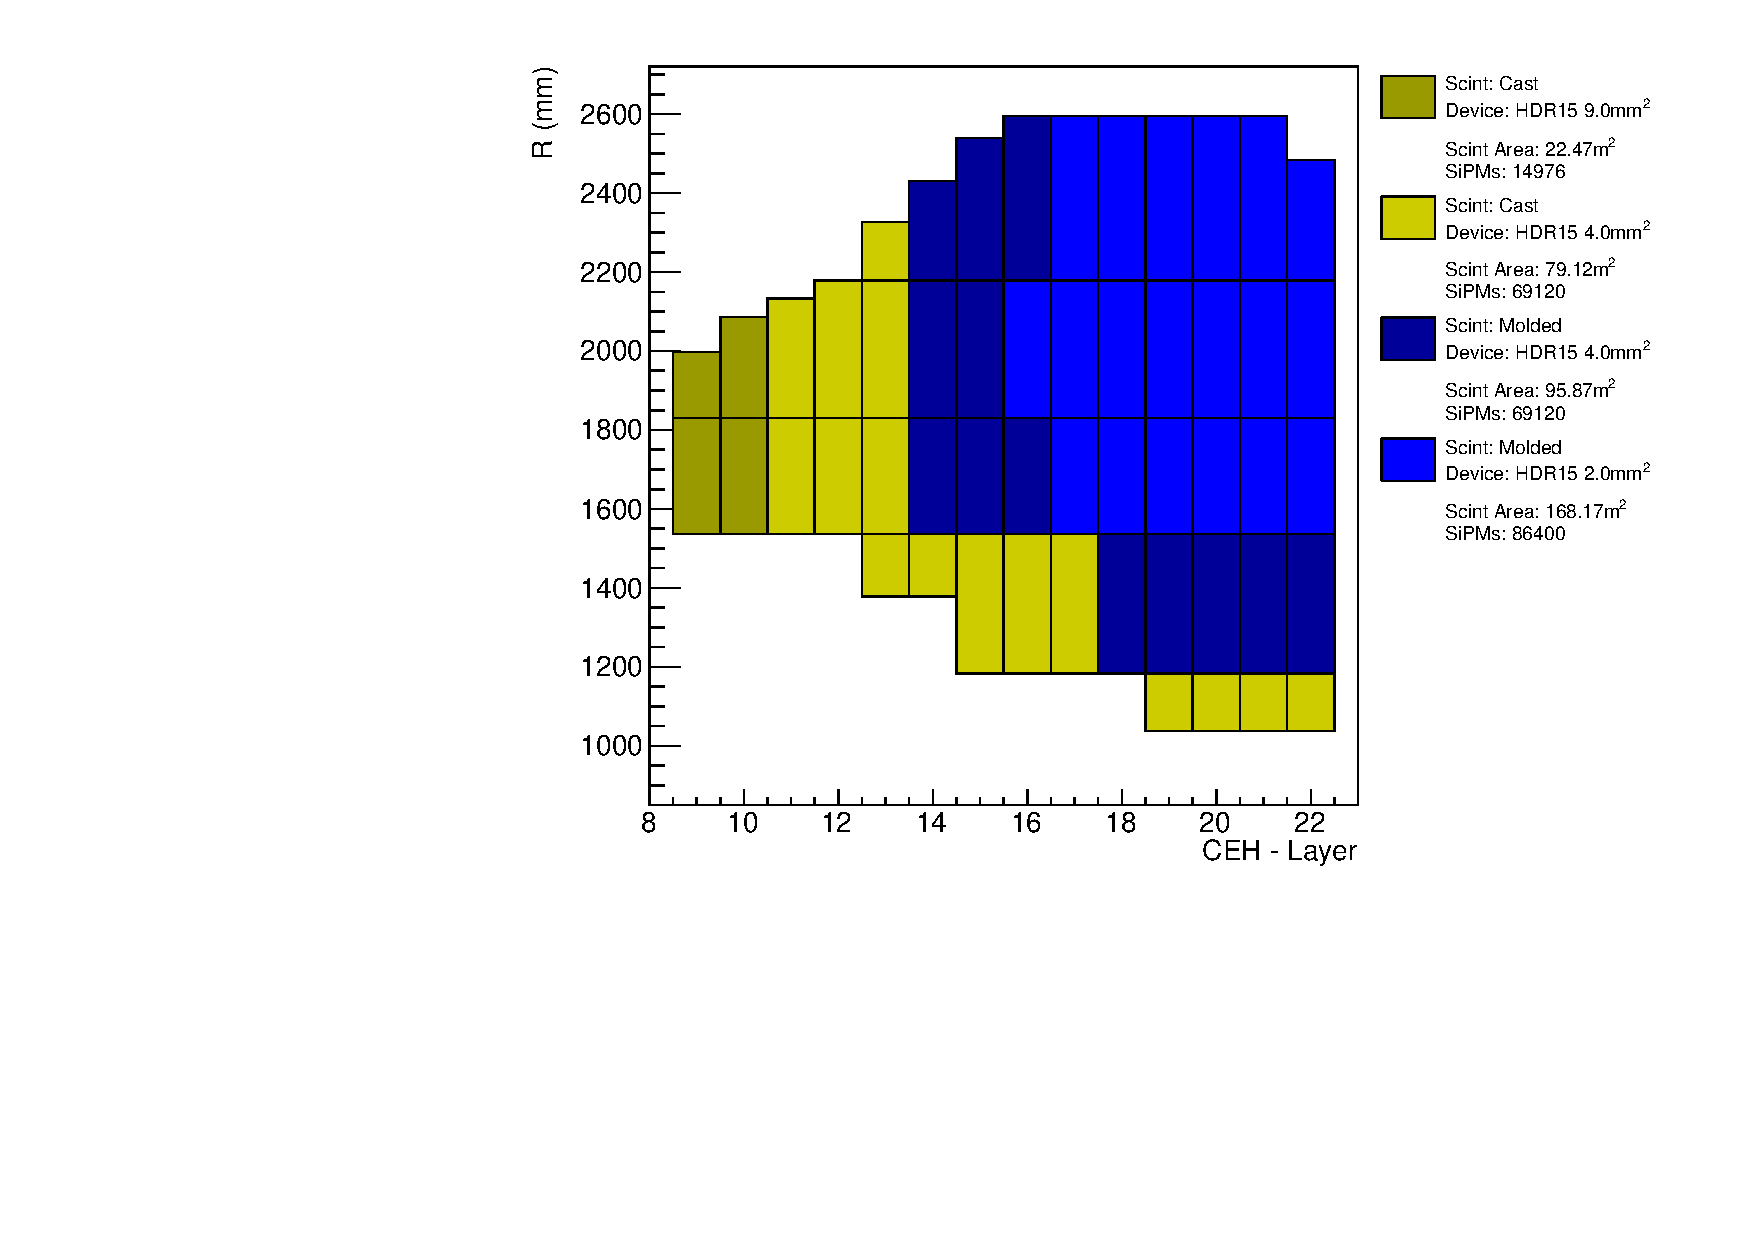
\includegraphics[trim={400 250 20 130},clip,width=0.24\textwidth]{figures/hgcal/plot_scenes/sceneA_jan20_fix_vto2p0_with9mm2.pdf}
  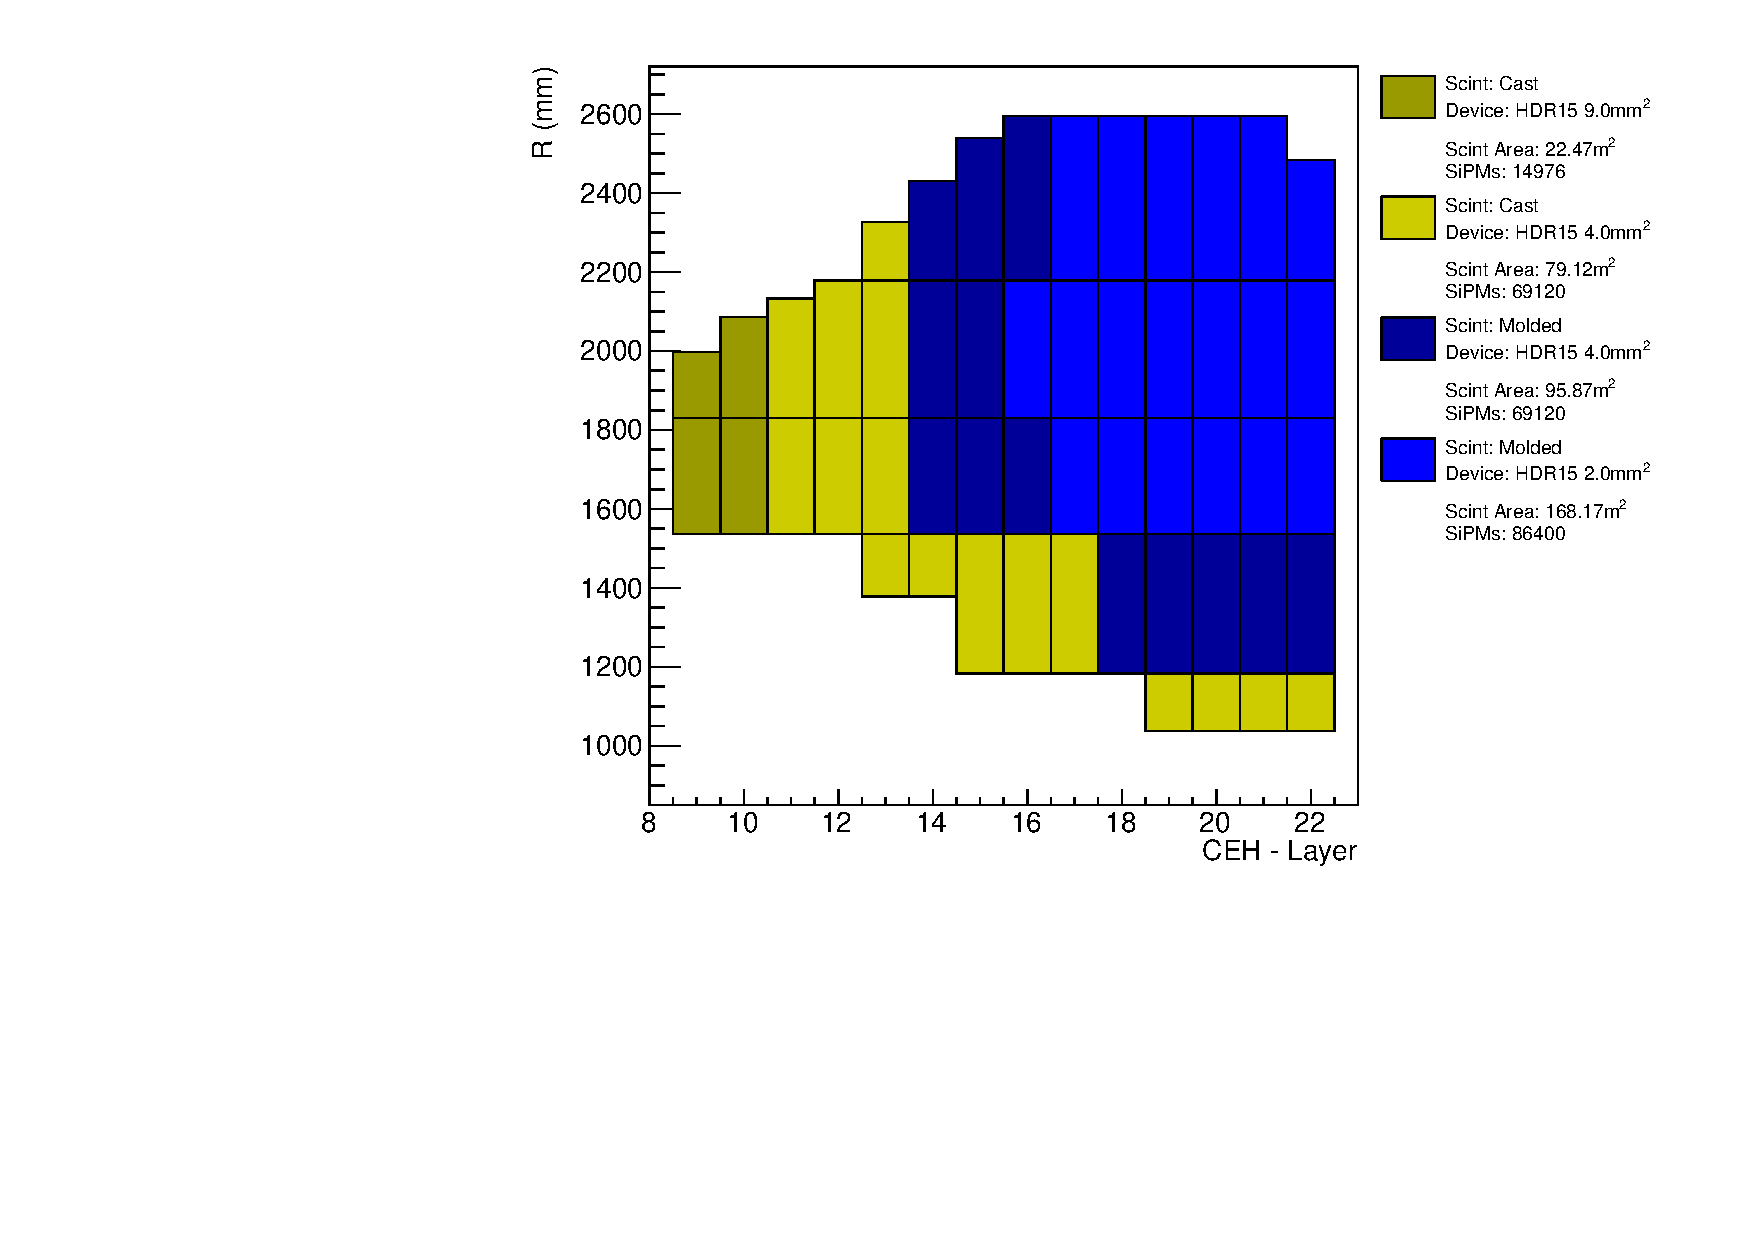
\includegraphics[trim={400 190 20 190},clip,width=0.24\textwidth]{figures/hgcal/plot_scenes/sceneA_jan20_fix_vto2p0_with9mm2.pdf}
  \begin{minipage}[c]{0.49\textwidth}
    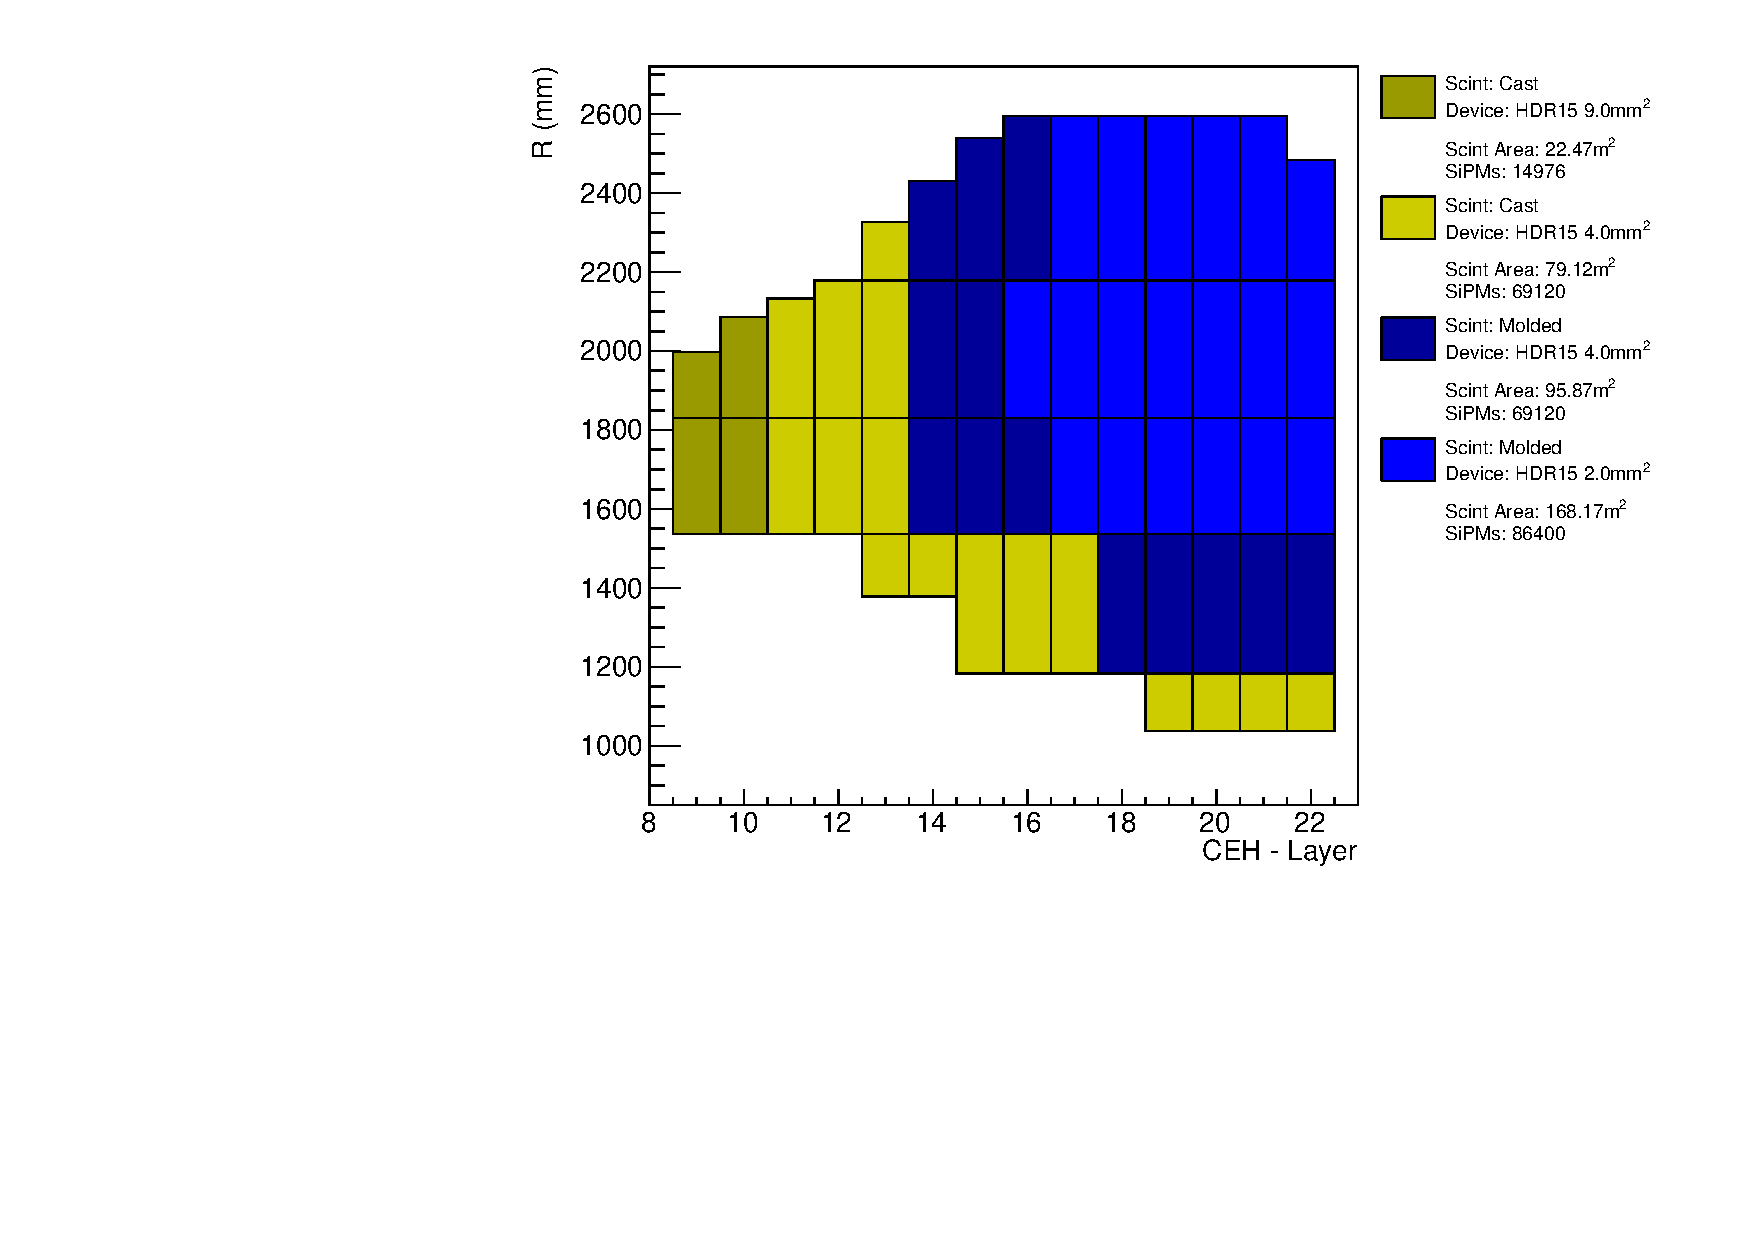
\includegraphics[trim={0 0 165pt 0},clip,width=\textwidth]{figures/hgcal/plot_scenes/sceneA_jan20_fix_vto2p0_with9mm2.pdf}
  \end{minipage}
  \begin{minipage}[c]{0.49\textwidth}
    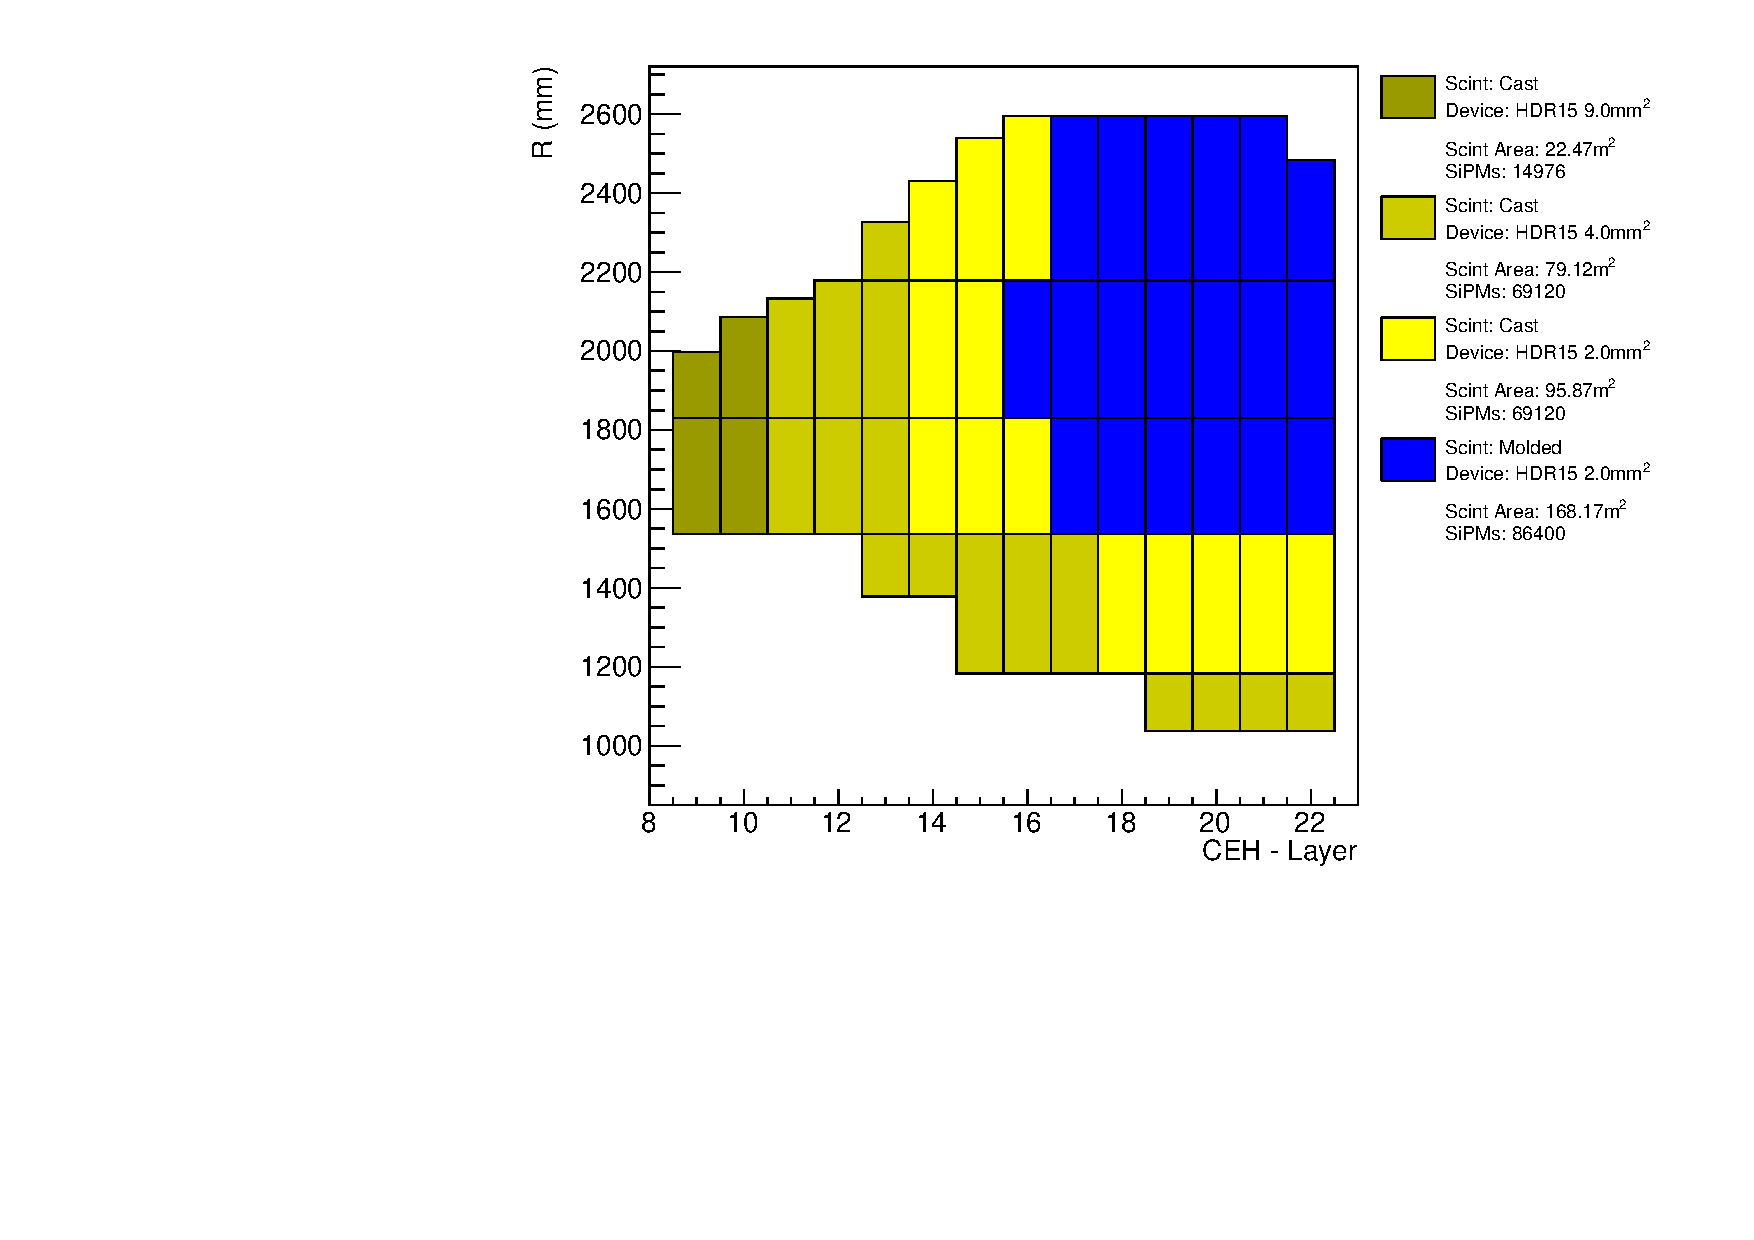
\includegraphics[trim={0 0 165pt 0},clip,width=\textwidth]{figures/hgcal/plot_scenes/sceneB_jan20_fix_vto2p0_with9mm2.pdf}
  \end{minipage}
  \caption[\gls{HGCAL} scenarios]{\gls{HGCAL} scenarios. Left: Scene A, Right: Scene B}%
  \label{fig:hgcal-scenes-fnal-jan20}
\end{figure}

\begin{table}[!ht]
  \centering
  \caption{\gls{HGCAL} scenarios comparison}
  \begin{tabular}{p{1.5in}cll}%
    \toprule
                                                   &                    & Scene A                & Scene B                \\
    \midrule
    \multirow{3}{=}{Cast Scintillator}             & Cell Count         & 84, 096                & 153,216                \\
                                                   & Total Area         & 101.59 \(\text{m}^2 \) & 197.46 \(\text{m}^2 \) \\
                                                   & Percentage         & 27.8 \%                & 54.0 \%                \\
    \cmidrule(lr){2-4}
    \multirow{3}{=}{Injection Molded Scintillator} & Cell Count         & 155, 520               & 63, 360                \\
                                                   & Total Area         & 264.04 \(\text{m}^2 \) & 168.17 \(\text{m}^2 \) \\
                                                   & Percentage         & 72.2 \%                & 46.0 \%                \\
    \cmidrule(lr){2-4}
    \multirow{2}{=}{SiPMs Count}                   & 2 \(\text{mm}^2 \) & 86, 400                & 69, 120                \\
                                                   & 4 \(\text{mm}^2 \) & 138, 240               & 155, 520               \\
                                                   & 9 \(\text{mm}^2 \) & 14, 976                & 14, 976                \\
    \bottomrule
  \end{tabular}
\end{table}